\documentclass[10pt]{article}
\usepackage[T1]{fontenc}
\usepackage[utf8]{inputenc}
%\DeclareUnicodeCharacter{00A0}{ }
\usepackage[adobe-utopia]{mathdesign}

\usepackage{amsmath}
\usepackage[francais]{babel}
\usepackage[dvips]{graphicx}
%\usepackage{here}
\usepackage{framed}
\usepackage[normalem]{ulem}
\usepackage{fancyhdr}
\usepackage{titlesec}
\usepackage{vmargin}

\usepackage{amsmath}
\usepackage{ifthen}
\usepackage{multirow}
\usepackage{multicol} % Portions de texte en colonnes

%\usepackage{xltxtra} % Logo XeLaTeX
%\usepackage{pst-solides3d}
\usepackage{color}
%\usepackage{colortbl}
\usepackage{titletoc} % Pour la mise en forme de la table des matières

%\usepackage[crop=off]{auto-pst-pdf}
%\usepackage{bclogo}


%\usepackage{longtable}
%\usepackage{flafter}%floatants après la référence
%\usepackage{pst-solides3d}
%\usepackage{pstricks}
%\usepackage{minitoc}
%\setcounter{minitocdepth}{4}
%\usepackage{draftcopy}% "Brouillon"
%\usepackage{floatflt}
%\usepackage{psfrag}
%\usepackage{listings} % Permet d'insérer du code de programmation
%\usepackage{lmodern}
%\usepackage[adobe-utopia,uppercase=upright,greeklowercase=upright]{mathdesign}
%\usepackage{minionpro}
%\usepackage{pifont}
%\usepackage{amssymb}
%\usepackage[francais]{varioref}

\setmarginsrb{1.5cm}{1cm}{1cm}{1.5cm}{1cm}{1cm}{1cm}{1cm}

\definecolor{gris25}{gray}{0.75}
\definecolor{bleu}{RGB}{18,33,98}
\definecolor{bleuf}{RGB}{42,94,171}
\definecolor{bleuc}{RGB}{231,239,247}
\definecolor{rougef}{RGB}{185,18,27}
\definecolor{rougec}{RGB}{255,230,231}
\definecolor{vertf}{RGB}{103,126,82}
\definecolor{vertc}{RGB}{220,255,191}
\definecolor{violetf}{RGB}{112,48,160}
\definecolor{violetc}{RGB}{230,224,236}
\definecolor{jaunec}{RGB}{220,255,191}
%\usepackage{algorithm}
%\usepackage{algorithmic}
\usepackage[french]{algorithm2e}

\SetKwBlock{Fonction}{Début Fonction}{Fin Fonction}
\SetKwComment{Comment}{start}{end}
% Python sources

\usepackage{listings}
\lstloadlanguages{R}   % pour regler les pb d accent utf8 dans les codes
\lstset{language=R} % pour regler les pb d accent utf8 dans les codes

\usepackage{textcomp}
\usepackage{setspace}
%\usepackage{palatino}

%\usepackage{color}
\definecolor{Bleu}{rgb}{0.1,0.1,1.0}
\definecolor{Noir}{rgb}{0,0,0}
\definecolor{Grau}{rgb}{0.5,0.5,0.5}
\definecolor{DunkelGrau}{rgb}{0.15,0.15,0.15}
\definecolor{Hellbraun}{rgb}{0.5,0.25,0.0}
\definecolor{Magenta}{rgb}{1.0,0.0,1.0}
\definecolor{Gris}{gray}{0.5}
\definecolor{Vert}{rgb}{0,0.5,0}
\definecolor{SourceHintergrund}{rgb}{1,1.0,0.95}


%
\renewcommand{\lstlistlistingname}{Listings}
\renewcommand{\lstlistingname}{Listing}

\lstnewenvironment{python}[1][]{
\lstset{
%escapeinside={\%*}{*)},
%inputencoding=utf8,   % pour regler les pb d accent utf8 dans les codes
%extendedchars=true,   % pour regler les pb d accent utf8 dans les codes
language=python,
basicstyle=\sffamily\footnotesize, 	
stringstyle=\color{red}, 
showstringspaces=false, 
alsoletter={1234567890},
otherkeywords={\ , \}, \{},
keywordstyle=\color{blue},
emph={access,and,break,class,continue,def,del,elif ,else,
except,exec,finally,for,from,global,if,import,in,i s,
lambda,not,or,pass,print,raise,return,try,while},
emphstyle=\color{black}\bfseries,
emph={[2]True, False, None, self},
emphstyle=[2]\color{olive},
emph={[3]from, import, as},
emphstyle=[3]\color{blue},
upquote=true,
columns=flexible, % pour empecher d'avoir un espacement mono
morecomment=[s]{"""}{"""},
commentstyle=\color{Hellbraun}\slshape, 
%emph={[4]1, 2, 3, 4, 5, 6, 7, 8, 9, 0},
emphstyle=[4]\color{blue},
literate=*{:}{{\textcolor{blue}:}}{1}
{=}{{\textcolor{blue}=}}{1}
{-}{{\textcolor{blue}-}}{1}
{+}{{\textcolor{blue}+}}{1}
{*}{{\textcolor{blue}*}}{1}
{!}{{\textcolor{blue}!}}{1}
{(}{{\textcolor{blue}(}}{1}
{)}{{\textcolor{blue})}}{1}
{[}{{\textcolor{blue}[}}{1}
{]}{{\textcolor{blue}]}}{1}
{<}{{\textcolor{blue}<}}{1}
{>}{{\textcolor{blue}>}}{1}
{COMPLETER}{{\textcolor{red}COMPLETER}}{1},
literate=%
            {é}{{\'{e}}}1
            {è}{{\`{e}}}1
            {ê}{{\^{e}}}1
            {ë}{{\¨{e}}}1
            {û}{{\^{u}}}1
            {ù}{{\`{u}}}1
            {â}{{\^{a}}}1
            {à}{{\`{a}}}1
            {î}{{\^{i}}}1
            {ç}{{\c{c}}}1
            {Ç}{{\c{C}}}1
            {É}{{\'{E}}}1
            {Ê}{{\^{E}}}1
            {À}{{\`{A}}}1
            {Â}{{\^{A}}}1
            {Î}{{\^{I}}}1, % pour regler les pb d accent utf8 dans les codes
%framexleftmargin=1mm, framextopmargin=1mm, frame=shadowbox, rulesepcolor=\color{blue},#1
%backgroundcolor=\color{SourceHintergrund}, 
%framexleftmargin=1mm, framexrightmargin=1mm, framextopmargin=1mm, frame=single, framerule=1pt, rulecolor=\color{black},#1
}}{}



\lstnewenvironment{scilab}[1][]{
\lstset{
language=scilab,
basicstyle=\sffamily\footnotesize, 	
stringstyle=\color{red}, 
showstringspaces=false, 
alsoletter={1234567890},
otherkeywords={\ , \}, \{},
keywordstyle=\color{blue},
emph={access,and,break,class,continue,def,del,elif ,else,
except,exec,finally,for,from,global,if,import,in,i s,
lambda,not,or,pass,print,raise,return,try,while,Debut},
emphstyle=\color{black}\bfseries,
emph={[2]True, False, None, self},
emphstyle=[2]\color{olive},
emph={[3]from, import, as},
emphstyle=[3]\color{blue},
upquote=true,
columns=flexible, % pour empecher d'avoir un espacement mono
morecomment=[s]{"""}{"""},
commentstyle=\color{Hellbraun}\slshape, 
%emph={[4]1, 2, 3, 4, 5, 6, 7, 8, 9, 0},
emphstyle=[4]\color{blue},
literate=*{:}{{\textcolor{blue}:}}{1}
{=}{{\textcolor{blue}=}}{1}
{-}{{\textcolor{blue}-}}{1}
{+}{{\textcolor{blue}+}}{1}
{*}{{\textcolor{blue}*}}{1}
{!}{{\textcolor{blue}!}}{1}
{(}{{\textcolor{blue}(}}{1}
{)}{{\textcolor{blue})}}{1}
{[}{{\textcolor{blue}[}}{1}
{]}{{\textcolor{blue}]}}{1}
{<}{{\textcolor{blue}<}}{1}
{>}{{\textcolor{blue}>}}{1},
%framexleftmargin=1mm, framextopmargin=1mm, frame=shadowbox, rulesepcolor=\color{blue},#1
%backgroundcolor=\color{SourceHintergrund}, 
%framexleftmargin=1mm, framexrightmargin=1mm, framextopmargin=1mm, frame=single, framerule=1pt, rulecolor=\color{black},#1
}}{}


\lstdefinestyle{stylepython}{%
escapeinside={\%*}{*)},
inputencoding=utf8,   % pour regler les pb d accent utf8 dans les codes
extendedchars=true,   % pour regler les pb d accent utf8 dans les codes
language=python,
basicstyle=\sffamily\footnotesize, 	
stringstyle=\color{red}, 
showstringspaces=false, 
alsoletter={1234567890},
otherkeywords={\ , \}, \{},
keywordstyle=\color{blue},
emph={access,and,break,class,continue,def,del,elif ,else,
except,exec,finally,for,from,global,if,import,in,i s,
lambda,not,or,pass,print,raise,return,try,while},
emphstyle=\color{black}\bfseries,
emph={[2]True, False, None, self},
emphstyle=[2]\color{green},
emph={[3]from, import, as},
emphstyle=[3]\color{blue},
upquote=true,
columns=flexible, % pour empecher d'avoir un espacement mono
morecomment=[s]{"""}{"""},
commentstyle=\color{Hellbraun}\slshape, 
%emph={[4]1, 2, 3, 4, 5, 6, 7, 8, 9, 0},
emphstyle=[4]\color{blue},
literate=*{:}{{\textcolor{blue}:}}{1}
{=}{{\textcolor{blue}=}}{1}
{-}{{\textcolor{blue}-}}{1}
{+}{{\textcolor{blue}+}}{1}
{*}{{\textcolor{blue}*}}{1}
{!}{{\textcolor{blue}!}}{1}
{(}{{\textcolor{blue}(}}{1}
{)}{{\textcolor{blue})}}{1}
{[}{{\textcolor{blue}[}}{1}
{]}{{\textcolor{blue}]}}{1}
{<}{{\textcolor{blue}<}}{1}
{>}{{\textcolor{blue}>}}{1}
{COMPLETER}{{\textcolor{red}COMPLETER}}{1},
literate=%
            {é}{{\'{e}}}1
            {è}{{\`{e}}}1
            {ê}{{\^{e}}}1
            {ë}{{\¨{e}}}1
            {û}{{\^{u}}}1
            {ù}{{\`{u}}}1
            {â}{{\^{a}}}1
            {à}{{\`{a}}}1
            {î}{{\^{i}}}1
            {ç}{{\c{c}}}1
            {Ç}{{\c{C}}}1
            {É}{{\'{E}}}1
            {Ê}{{\^{E}}}1
            {À}{{\`{A}}}1
            {Â}{{\^{A}}}1
            {Î}{{\^{I}}}1,
%numbers=left,                    % where to put the line-numbers; possible values are (none, left, right)
%numbersep=5pt,                   % how far the line-numbers are from the code
%numberstyle=\tiny\color{mygray}, % the style that is used for the line-numbers
}

%
%\renewcommand{\algorithmicrequire} {\textbf{\textsc{Entrées:}}}
%\renewcommand{\algorithmicensure}  {\textbf{\textsc{Sorties:}}}
%\renewcommand{\algorithmicwhile}   {\textbf{tantque}}
%\renewcommand{\algorithmicdo}      {\textbf{faire}}
%\renewcommand{\algorithmicendwhile}{\textbf{fin tantque}}
%\renewcommand{\algorithmicend}     {\textbf{fin}}
%\renewcommand{\algorithmicif}      {\textbf{si}}
%\renewcommand{\algorithmicendif}   {\textbf{finsi}}
%\renewcommand{\algorithmicelse}    {\textbf{sinon}}
%\renewcommand{\algorithmicthen}    {\textbf{alors}}
%\renewcommand{\algorithmicfor}     {\textbf{pour}}
%\renewcommand{\algorithmicforall}  {\textbf{pour tout}}
%\renewcommand{\algorithmicdo}      {\textbf{faire}}
%\renewcommand{\algorithmicendfor}  {\textbf{fin pour}}
%\renewcommand{\algorithmicloop}    {\textbf{boucler}}
%\renewcommand{\algorithmicendloop} {\textbf{fin boucle}}
%\renewcommand{\algorithmicrepeat}  {\textbf{répéter}}
%\renewcommand{\algorithmicuntil}   {\textbf{jusqu'à}}

\lstnewenvironment{termi}[1][]{
\lstset{
language=scilab,
basicstyle=\sffamily\footnotesize, 	
stringstyle=\color{red}, 
showstringspaces=false, 
alsoletter={1234567890},
otherkeywords={\ , \}, \{},
keywordstyle=\color{blue},
emph={access,and,break,class,continue,def,del,elif ,else,
except,exec,finally,for,from,global,if,import,in,i s,
lambda,not,or,pass,print,raise,return,try,while,Debut},
emphstyle=\color{black}\bfseries,
emph={[2]True, False, None, self},
emphstyle=[2]\color{green},
emph={[3]from, import, as},
emphstyle=[3]\color{blue},
upquote=true,
columns=flexible, % pour empecher d'avoir un espacement mono
morecomment=[s]{"""}{"""},
commentstyle=\color{Hellbraun}\slshape, 
%emph={[4]1, 2, 3, 4, 5, 6, 7, 8, 9, 0},
emphstyle=[4]\color{blue},
literate=*{:}{{\textcolor{blue}:}}{1}
{=}{{\textcolor{blue}=}}{1}
{-}{{\textcolor{blue}-}}{1}
{+}{{\textcolor{blue}+}}{1}
{*}{{\textcolor{blue}*}}{1}
{!}{{\textcolor{blue}!}}{1}
{(}{{\textcolor{blue}(}}{1}
{)}{{\textcolor{blue})}}{1}
{[}{{\textcolor{blue}[}}{1}
{]}{{\textcolor{blue}]}}{1}
{<}{{\textcolor{blue}<}}{1}
{>}{{\textcolor{blue}>}}{1},
%framexleftmargin=1mm, framextopmargin=1mm, frame=shadowbox, rulesepcolor=\color{blue},#1
%backgroundcolor=\color{SourceHintergrund}, 
%framexleftmargin=1mm, framexrightmargin=1mm, framextopmargin=1mm, frame=single, framerule=1pt, rulecolor=\color{black},#1
}}{}


%
%\renewcommand{\algorithmicrequire} {\textbf{\textsc{Entrées:}}}
%\renewcommand{\algorithmicensure}  {\textbf{\textsc{Sorties:}}}
%\renewcommand{\algorithmicwhile}   {\textbf{tantque}}
%\renewcommand{\algorithmicdo}      {\textbf{faire}}
%\renewcommand{\algorithmicendwhile}{\textbf{fin tantque}}
%\renewcommand{\algorithmicend}     {\textbf{fin}}
%\renewcommand{\algorithmicif}      {\textbf{si}}
%\renewcommand{\algorithmicendif}   {\textbf{finsi}}
%\renewcommand{\algorithmicelse}    {\textbf{sinon}}
%\renewcommand{\algorithmicthen}    {\textbf{alors}}
%\renewcommand{\algorithmicfor}     {\textbf{pour}}
%\renewcommand{\algorithmicforall}  {\textbf{pour tout}}
%\renewcommand{\algorithmicdo}      {\textbf{faire}}
%\renewcommand{\algorithmicendfor}  {\textbf{fin pour}}
%\renewcommand{\algorithmicloop}    {\textbf{boucler}}
%\renewcommand{\algorithmicendloop} {\textbf{fin boucle}}
%\renewcommand{\algorithmicrepeat}  {\textbf{répéter}}
%\renewcommand{\algorithmicuntil}   {\textbf{jusqu'à}}
%%%%%%%%%%%%
% Définition des vecteurs 
%%%%%%%%%%%%
 \newcommand{\vect}[1]{\overrightarrow{#1}}
\newcommand{\axe}[2]{\left(#1,\vect{#2}\right)}

\newcommand{\rep}[1]{\mathcal{R}_{#1}}
\newcommand{\vx}[1]{\vect{x_{#1}}}
\newcommand{\vy}[1]{\vect{y_{#1}}}
\newcommand{\vz}[1]{\vect{z_{#1}}}

%%%%%%%%%%%%
% Définition des torseurs 
%%%%%%%%%%%%

 \newcommand{\torseur}[1]{%
\left\{{#1}\right\}
}

\newcommand{\torseurcin}[3]{%
\left\{\mathcal{#1} \left(#2/#3 \right) \right\}
}

\newcommand{\torseurstat}[3]{%
\left\{\mathcal{#1} \left(#2\rightarrow #3 \right) \right\}
}

 \newcommand{\torseurc}[8]{%
%\left\{#1 \right\}=
\left\{
{#1}
\right\}
 = 
\left\{%
\begin{array}{cc}%
{#2} & {#5}\\%
{#3} & {#6}\\%
{#4} & {#7}\\%
\end{array}%
\right\}_{#8}%
}

 \newcommand{\torseurcol}[7]{
\left\{%
\begin{array}{cc}%
{#1} & {#4}\\%
{#2} & {#5}\\%
{#3} & {#6}\\%
\end{array}%
\right\}_{#7}%
}

 \newcommand{\torseurl}[3]{%
%\left\{\mathcal{#1}\right\}_{#2}=%
\left\{%
\begin{array}{l}%
{#1} \\%
{#2} %
\end{array}%
\right\}_{#3}%
}

 \newcommand{\vectv}[3]{%
\vect{V\left( {#1} \in {#2}/{#3}\right)}
}


\newcommand{\vectf}[2]{%
\vect{R\left( {#1} \rightarrow {#2}\right)}
}

\newcommand{\vectm}[3]{%
\vect{\mathcal{M}\left( {#1}, {#2} \rightarrow {#3}\right)}
}


 \newcommand{\vectg}[3]{%
\vect{\Gamma \left( {#1} \in {#2}/{#3}\right)}
}

 \newcommand{\vecto}[2]{%
\vect{\Omega\left( {#1}/{#2}\right)}
}
% }$$\left\{\mathcal{#1} \right\}_{#2} =%
% \left\{%
% \begin{array}{c}%
%  #3 \\%
%  #4 %
% \end{array}%
% \right\}_{#5}}
\setcounter{tocdepth}{2}
% \mtcselectlanguage{french} 


%  ------------------------------------------
% | Modification du formatage des sections : | 
%  ------------------------------------------

% Grands titres :
% ---------------

\newcommand{\titre}[1]{%
\begin{center}
      \bigskip
      \rule{\textwidth}{1pt}
      \par\vspace{0.1cm}
      
      \textbf{\large #1}
      \par\rule{\textwidth}{1pt}
    \end{center}
    \bigskip
  }

% Supprime le numéro du chapitre dans la numérotation des sections:
% -----------------------------------------------------------------
\makeatletter
\renewcommand{\thesection}{\@arabic\c@section}
\makeatother


% \titleformat{\chapter}[display]
% {\normalfont\Large\filcenter}
% {}
% {1pc}
% {\titlerule[1pt]
%   \vspace{1pc}%
%   \Huge}[\vspace{1ex}%
% \titlerule]


%%%% Chapitres Comme PY Pechard %%%%%%%%%
% numéro du chapitre
\DeclareFixedFont{\chapnumfont}{OT1}{phv}{b}{n}{80pt}
% pour le mot « Chapitre »
\DeclareFixedFont{\chapchapfont}{OT1}{phv}{m}{it}{40pt}
% pour le titre
\DeclareFixedFont{\chaptitfont}{T1}{phv}{b}{n}{25pt}

\definecolor{gris}{gray}{0.75}
\titleformat{\chapter}[display]%
	{\sffamily}%
	{\filleft\chapchapfont\color{gris}\chaptertitlename\
	\\
	\vspace{12pt}
	\chapnumfont\thechapter}%
	{16pt}%
	{\filleft\chaptitfont}%
	[\vspace{6pt}\titlerule\titlerule\titlerule]

%%%%  Fin Chapitres Comme PY Pechard %%%%%%%%%


% Section, subsection, subsubsection sans serifs :
% % ----------------------------------------------

% \makeatletter
% \renewcommand{\section}{\@startsection{section}{0}{0mm}%
% {\baselineskip}{.3\baselineskip}%
% {\normalfont\sffamily\Large\textbf}}%
% \makeatother

\makeatletter
\renewcommand{\@seccntformat}[1]{{\textcolor{bleu}{\csname
the#1\endcsname}\hspace{0.5em}}}
\makeatother

\makeatletter
\renewcommand{\section}{\@startsection{section}{1}{\z@}%
                       {-4ex \@plus -1ex \@minus -.4ex}%
                       {1ex \@plus.2ex }%
                       {\normalfont\Large\sffamily\bfseries}}%
\makeatother
 
\makeatletter
\renewcommand{\subsection}{\@startsection {subsection}{2}{\z@}
                          {-3ex \@plus -0.1ex \@minus -.4ex}%
                          {0.5ex \@plus.2ex }%
                          {\normalfont\large\sffamily\bfseries}}
\makeatother
 
\makeatletter
\renewcommand{\subsubsection}{\@startsection {subsubsection}{3}{\z@}
                          {-2ex \@plus -0.1ex \@minus -.2ex}%
                          {0.2ex \@plus.2ex }%
                          {\normalfont\large\sffamily\bfseries}}
\makeatother
 
\makeatletter             
\renewcommand{\paragraph}{\@startsection{paragraph}{4}{\z@}%
                                    {-2ex \@plus-.2ex \@minus .2ex}%
                                    {0.1ex}%               
{\normalfont\sffamily\bfseries}}
\makeatother
 
 
\makeatletter             
\renewcommand{\subparagraph}{\@startsection{subparagraph}{5}{\z@}%
                                    {-2ex \@plus-.2ex \@minus .2ex}%
                                    {0.1ex}%               
{\normalfont\bfseries Question }}
\makeatother
\renewcommand{\thesubparagraph}{\arabic{subparagraph}} 
\makeatletter

\setcounter{secnumdepth}{5}





% Formatage de la table des matières 
% Paquets nécessaires : titletoc ?

% Chapitre spéciaux écrits dans un nombre cerclé dans la table des matières.
\titlecontents{chapter}[+3pc]
  {\addvspace{10pt}\sffamily\bfseries}
{\contentslabel[{\pscirclebox[fillstyle=solid,fillcolor=gray!25,
linecolor=gray!25,framesep=4pt]{\textcolor{white}{\thecontentslabel}}}]{2.5pc}}
  {}
  {\dotfill \normalfont\thecontentspage\ }

\titlecontents{section}[3pc]
  {\addvspace{2pt}\sffamily}
  {\contentslabel[\thecontentslabel]{1.8pc}}
  {}
  {\dotfill \normalfont\thecontentspage\ }

\titlecontents{subsection}[5pc]
  {\addvspace{2pt}\sffamily}
  {\contentslabel[\thecontentslabel]{1.8pc}}
  {}
  {\dotfill \normalfont\thecontentspage\ }

\titlecontents{subsubsection}[8pc]
  {\addvspace{2pt}\sffamily}
  {\contentslabel[\thecontentslabel]{3pc}}
  {}
  {\dotfill \normalfont\thecontentspage\ }
%{\;\titlerule\;\normalfont\thecontentspage\ }

\titlecontents{paragraph}[9pc]
  {\addvspace{2pt}\sffamily}
  {\contentslabel[\thecontentslabel]{3.5pc}}
  {}
  {\dotfill \normalfont\thecontentspage\ }

%pour avoir l indentation dans minipage
\newdimen\oldparindent\oldparindent=\parindent

\makeatletter
\def\@iiiminipage#1#2[#3]#4{%
  \noindent
  \leavevmode
  \@pboxswfalse
  \setlength\@tempdima{#4}%
  \def\@mpargs{{#1}{#2}[#3]{#4}}%
  \setbox\@tempboxa\vbox\bgroup
    \color@begingroup
      \hsize\@tempdima
      \textwidth\hsize \columnwidth\hsize
      \@parboxrestore
      \parindent=\oldparindent
      \def\@mpfn{mpfootnote}\def\thempfn{\thempfootnote}\c@mpfootnote\z@
      \let\@footnotetext\@mpfootnotetext
      \let\@listdepth\@mplistdepth \@mplistdepth\z@
      \@minipagerestore
      \@setminipage}
\makeatother

% Paquets requis : 

\definecolor{gris25}{gray}{0.75}
\definecolor{bleu}{RGB}{18,33,98}
\definecolor{bleuf}{RGB}{42,94,171}
\definecolor{bleuc}{RGB}{231,239,247}
\definecolor{rougef}{RGB}{185,18,27}
\definecolor{rougec}{RGB}{255,230,231}
\definecolor{vertf}{RGB}{103,126,82}
\definecolor{vertc}{RGB}{220,255,191}
\definecolor{violetf}{RGB}{112,48,160}
\definecolor{violetc}{RGB}{230,224,236}
\definecolor{jaunec}{RGB}{220,255,191}



\newenvironment{corrige}[1][\hsize]%
{%
    \def\FrameCommand%
    {%
\rotatebox{90}{\textit{\textsf{Corrigé}}} 
        {\color{violetf}\vrule width 3pt}%
        \hspace{0pt}%must no space.
        \fboxsep=\FrameSep\colorbox{violetc}%
    }%
    \MakeFramed{\hsize #1 \advance\hsize-\width\FrameRestore}%
}%
{\endMakeFramed}%

\newenvironment{sci}[1][\hsize]%
{%
    \def\FrameCommand%
    {%
%\rotatebox{90}{\textit{\textsf{Scilab}}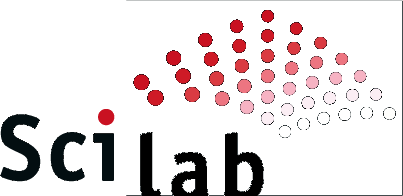
\includegraphics[height=.8cm]{png/logo_scilab}} 
\rotatebox{90}{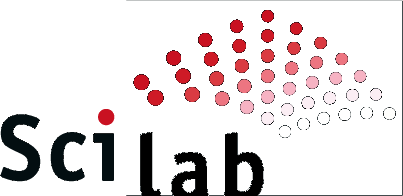
\includegraphics[height=.6cm]{png/logo_scilab}} 
        {\color{violetf}\vrule width 3pt}%
        \hspace{0pt}%must no space.
        \fboxsep=\FrameSep\colorbox{violetc}%
    }%
    \MakeFramed{\hsize #1 \advance\hsize-\width\FrameRestore}%
}%
{\endMakeFramed}%

\newenvironment{pseudo}[1][\hsize]%
{%
    \def\FrameCommand%
    {%
\rotatebox{90}{\textit{\textsf{Pseudo Code}}} 
        {\color{violetf}\vrule width 3pt}%
        \hspace{0pt}%must no space.
        \fboxsep=\FrameSep\colorbox{violetc}%
    }%
    \MakeFramed{\hsize #1 \advance\hsize-\width\FrameRestore}%
}%
{\endMakeFramed}%

\newenvironment{py}[1][\hsize]%
{%
    \def\FrameCommand%
    {%
%\rotatebox{90}{\textit{\textsf{Python}}} 
\rotatebox{90}{
\includegraphics[height=.6cm]{png/logo_python}} 
        {\color{violetf}\vrule width 3pt}%
        \hspace{0pt}%must no space.
        \fboxsep=\FrameSep\colorbox{violetc}%
    }%
    \MakeFramed{\hsize #1 \advance\hsize-\width\FrameRestore}%
}%
{\endMakeFramed}%


\newenvironment{term}[1][\hsize]%
{%
    \def\FrameCommand%
    {%
\rotatebox{90}{\textit{\textsf{Terminal}}} 
        {\color{violetf}\vrule width 3pt}%
        \hspace{0pt}%must no space.
        \fboxsep=\FrameSep\colorbox{violetc}%
    }%
    \MakeFramed{\hsize #1 \advance\hsize-\width\FrameRestore}%
}%
{\endMakeFramed}%



\newenvironment{comp}[1][\hsize]%
{%
    \def\FrameCommand
    {%
\rotatebox{90}{\textit{\textsf{Compétences}}} 
        {\color{bleuf}\vrule width 3pt}%
        \hspace{0pt}%must no space.
        \fboxsep=\FrameSep\colorbox{bleuc}%
    }%
    \MakeFramed{\hsize#1\advance\hsize-\width\FrameRestore}%
}%
{\endMakeFramed}%

\newenvironment{rem}[1][\hsize]%
{%
    \def\FrameCommand
    {%
\rotatebox{90}{\textit{\textsf{Remarque}}} 
        {\color{bleuf}\vrule width 3pt}%
        \hspace{0pt}%must no space.
        \fboxsep=\FrameSep\colorbox{bleuc}%
    }%
    \MakeFramed{\hsize#1\advance\hsize-\width\FrameRestore}%
}%
{\endMakeFramed}%


\newenvironment{savoir}[1][\hsize]%
{%
    \def\FrameCommand
    {%
\rotatebox{90}{\textit{\textsf{Savoir}}} 
        {\color{bleuf}\vrule width 3pt}%
        \hspace{0pt}%must no space.
        \fboxsep=\FrameSep\colorbox{bleuc}%
    }%
    \MakeFramed{\hsize#1\advance\hsize-\width\FrameRestore}%
}%
{\endMakeFramed}%

\newenvironment{Objectif}[1][\hsize]%
{%
    \def\FrameCommand
    {%
\rotatebox{90}{\textit{\textsf{Objectif}}} 
        {\color{bleuf}\vrule width 3pt}%
        \hspace{0pt}%must no space.
        \fboxsep=\FrameSep\colorbox{bleuc}%
    }%
    \MakeFramed{\hsize#1\advance\hsize-\width\FrameRestore}%
}%
{\endMakeFramed}%

\newenvironment{prob}[1][\hsize]%
{%
    \def\FrameCommand%
    {%
\rotatebox{90}{\textit{\textsf{ Problématique}}} 
        {\color{rougef}\vrule width 3pt}%
        \hspace{0pt}%must no space.
        \fboxsep=\FrameSep\colorbox{rougec}%
    }%
    \MakeFramed{\hsize#1\advance\hsize-\width\FrameRestore}%
}%
{\endMakeFramed}%

\newenvironment{obj}[1][\hsize]%
{%
    \def\FrameCommand%
    {%
\rotatebox{90}{\textit{\textsf{Objectifs}}} 
        {\color{rougef}\vrule width 3pt}%
        \hspace{0pt}%must no space.
        \fboxsep=\FrameSep\colorbox{rougec}%
    }%
    \MakeFramed{\hsize#1\advance\hsize-\width\FrameRestore}%
}%
{\endMakeFramed}%

\newenvironment{defi}[1][\hsize]%
{%
    \def\FrameCommand%
    {%
\rotatebox{90}{\textit{\textsf{Définition\\}}} 
        {\color{bleuf}\vrule width 3pt}%
        \hspace{0pt}%must no space.
        \fboxsep=\FrameSep\colorbox{bleuc}%
    }%
    \MakeFramed{\hsize#1\advance\hsize-\width\FrameRestore}%
}%
{\endMakeFramed}%


\newenvironment{demo}[1][\hsize]%
{%
    \def\FrameCommand%
    {%
\rotatebox{90}{\textit{\textsf{Démonstration\\}}} 
        {\color{bleuf}\vrule width 3pt}%
        \hspace{0pt}%must no space.
        \fboxsep=\FrameSep\colorbox{bleuc}%
    }%
    \MakeFramed{\hsize#1\advance\hsize-\width\FrameRestore}%
}%
{\endMakeFramed}%


\newenvironment{hypo}[1][\hsize]%
{%
    \def\FrameCommand%
    {%
\rotatebox{90}{\textit{\textsf{Hypothèse\\}}} 
        {\color{bleuf}\vrule width 3pt}%
        \hspace{0pt}%must no space.
        \fboxsep=\FrameSep\colorbox{bleuc}%
    }%
    \MakeFramed{\hsize#1\advance\hsize-\width\FrameRestore}%
}%
{\endMakeFramed}%


\newenvironment{prop}[1][\hsize]%
{%
    \def\FrameCommand%
    {%
\rotatebox{90}{\textit{\textsf{Propriété\\}}} 
        {\color{bleuf}\vrule width 3pt}%
        \hspace{0pt}%must no space.
        \fboxsep=\FrameSep\colorbox{bleuc}%
    }%
    \MakeFramed{\hsize#1\advance\hsize-\width\FrameRestore}%
}%
{\endMakeFramed}%

\newenvironment{props}[1][\hsize]%
{%
    \def\FrameCommand%
    {%
\rotatebox{90}{\textit{\textsf{Propriétés\\}}} 
        {\color{bleuf}\vrule width 3pt}%
        \hspace{0pt}%must no space.
        \fboxsep=\FrameSep\colorbox{bleuc}%
    }%
    \MakeFramed{\hsize#1\advance\hsize-\width\FrameRestore}%
}%
{\endMakeFramed}%

\newenvironment{exemple}[1][\hsize]%
{%
    \def\FrameCommand%
    {%
\rotatebox{90}{\textit{\textsf{Exemple\\}}} 
        {\color{vertf}\vrule width 3pt}%
        \hspace{0pt}%must no space.
        \fboxsep=\FrameSep\colorbox{vertc}%
    }%
    \MakeFramed{\hsize#1\advance\hsize-\width\FrameRestore}%
}%
{\endMakeFramed}%

\newenvironment{exercice}[1][\hsize]%
{%
    \def\FrameCommand%
    {%
\rotatebox{90}{\textit{\textsf{Exercice\\}}} 
        {\color{vertf}\vrule width 3pt}%
        \hspace{0pt}%must no space.
        \fboxsep=\FrameSep\colorbox{vertc}%
    }%
    \MakeFramed{\hsize#1\advance\hsize-\width\FrameRestore}%
}%
{\endMakeFramed}%

\newenvironment{Support}[1][\hsize]%
{%
    \def\FrameCommand%
    {%
\rotatebox{90}{\textit{\textsf{Support de cours\\}}} 
        {\color{vertf}\vrule width 3pt}%
        \hspace{0pt}%must no space.
        \fboxsep=\FrameSep\colorbox{jaunec}%
    }%
    \MakeFramed{\hsize#1\advance\hsize-\width\FrameRestore}%
}%
{\endMakeFramed}%

\newenvironment{resultat}[1][\hsize]%
{%
    \def\FrameCommand%
    {%
\rotatebox{90}{\textit{\textsf{Résultat\\}}} 
        {\color{rougef}\vrule width 3pt}%
        \hspace{0pt}%must no space.
        \fboxsep=\FrameSep\colorbox{rougec}%
    }%
    \MakeFramed{\hsize#1\advance\hsize-\width\FrameRestore}%
}%
{\endMakeFramed}%

\newenvironment{methode}[1][\hsize]%
{%
    \def\FrameCommand%
    {%
\rotatebox{90}{\textit{\textsf{Méthode\\}}} 
        {\color{rougef}\vrule width 3pt}%
        \hspace{0pt}%must no space.
        \fboxsep=\FrameSep\colorbox{rougec}%
    }%
    \MakeFramed{\hsize#1\advance\hsize-\width\FrameRestore}%
}%
{\endMakeFramed}%

\newenvironment{theo}[1][\hsize]%
{%
    \def\FrameCommand%
    {%
\rotatebox{90}{\textit{\textsf{Théorème\\}}} 
        {\color{rougef}\vrule width 3pt}%
        \hspace{0pt}%must no space.
        \fboxsep=\FrameSep\colorbox{rougec}%
    }%
    \MakeFramed{\hsize#1\advance\hsize-\width\FrameRestore}%
}%
{\endMakeFramed}%

\newenvironment{warn}[1][\hsize]%
{%
    \def\FrameCommand%
    {%
\rotatebox{90}{\textit{\textsf{Attention\\}}} 
        {\color{rougef}\vrule width 3pt}%
        \hspace{0pt}%must no space.
        \fboxsep=\FrameSep\colorbox{rougec}%
    }%
    \MakeFramed{\hsize#1\advance\hsize-\width\FrameRestore}%
}%
{\endMakeFramed}%

%Si le boolen xp est vrai : compilation pour xabi
%Sinon compilation Damien

\newif\ifprof
\proftrue
%\proffalse

\newif\ifxp
\xptrue
%\xpfalse

\newif\iftd
\tdtrue
%\tdfalse


\usepackage[%
    pdftitle={},
    pdfauthor={Xavier Pessoles},
    colorlinks=true,
    linkcolor=blue,
    citecolor=magenta]{hyperref}


\def\discipline{Sciences Industrielles de l'Ingénieur}
\def\xxtitre{%
\ifxp
07 Étude des systèmes mécaniques : Concevoir 
\else
\fi
}

\def\xxsoustitre{%
\ifxp
Grue hydraulique : Conception du treuil
\else
\fi}

\def\xxauteur{%
\ifxp
Xavier \textsc{Pessoles}
\else
\fi}

\def\xxpied{%
\ifxp
07 Étude des systèmes mécaniques : Concevoir \\
Conception d'un treuil hydraulique
\else
\fi}



%---------------------------------------------------------------------------


\begin{document}
\ifxp

\sloppy
\hyphenpenalty 10000


%------------- En tetes et Pieds de Pages ------------

\pagestyle{fancy}
\renewcommand{\headrulewidth}{0pt}
\fancyhead{}
\fancyhead[L]{%
\noindent\begin{minipage}[c]{2.6cm}%

\includegraphics[width=2cm]{png/logo_ptsi.png}%
\end{minipage}}


\fancyhead[C]{\rule{12cm}{.5pt}}


\fancyhead[R]{%
\noindent\begin{minipage}[c]{3cm}
\begin{flushright}
\footnotesize{\textit{\textsf{\discipline}}}%
\end{flushright}
\end{minipage}
}



\fancyhead[C]{\rule{12cm}{.5pt}}

\renewcommand{\footrulewidth}{0.2pt}

\fancyfoot[C]{\footnotesize{\bfseries \thepage}}
\fancyfoot[L]{%
\begin{minipage}[c]{.2\linewidth}
\noindent\footnotesize{{\xxauteur}}
\end{minipage}
}

\fancyfoot[R]{\footnotesize{\xxpied}}

\begin{center}
 \ifthenelse{\boolean{td}}{\Large\textsc{\xxtitre}}{\huge\textsc{\xxtitre}}
\end{center}

\begin{center}
 \ifthenelse{\boolean{td}}{\large\textsc{\xxsoustitre}}{ \LARGE\textsc{\xxsoustitre}}
\end{center}

\vspace{.5cm}

\else
\ifthenelse{\boolean{xp}}{
\usepackage[%
    pdftitle={OS et Environnement de développement},
    pdfauthor={Xavier Pessoles},
    colorlinks=true,
    linkcolor=blue,
    citecolor=magenta]{hyperref}}{
\usepackage[%
    pdftitle={OS et Environnement de développement},
    pdfauthor={Damien Iceta},
    colorlinks=true,
    linkcolor=blue,
    citecolor=magenta]{hyperref}}

\usepackage{pifont}
\usepackage{lastpage}

% \makeatletter \let\ps@plain\ps@empty \makeatother
%% DEBUT DU DOCUMENT
%% =================
\sloppy
\hyphenpenalty 10000

\newcommand{\Pointilles}[1][3]{%
\multido{}{#1}{\makebox[\linewidth]{\dotfill}\\[\parskip]
}}


\colorlet{shadecolor}{orange!15}

\newtheorem{theorem}{Theorem}


\begin{document}


\newboolean{prof}
\setboolean{prof}{true}
%------------- En tetes et Pieds de Pages ------------


\pagestyle{fancy}
%\renewcommand{\headrulewidth}{0}
\renewcommand{\headrulewidth}{0.2pt} %pour mettre le trait en haut

\fancyhead{}
\fancyhead[L]{
\footnotesize{{{\xxtitre}}}%
%\noindent\noindent\begin{minipage}[c]{2.6cm}
%\includegraphics[width=2.5cm]{png/logo.png}%
%\end{minipage}
}

%\fancyhead[C]{\rule{12cm}{.5pt}}  %pour mettre le petit trait en haut


\fancyhead[R]{%
\noindent\begin{minipage}[c]{3cm}
\begin{flushright}
\footnotesize{{{\xxcathegorie}}}%
\end{flushright}
\end{minipage}
}

\renewcommand{\footrulewidth}{0.2pt}

\fancyfoot[C]{\footnotesize{}}
\fancyfoot[L]{%
\begin{minipage}[l]{.2\linewidth}
\noindent\footnotesize{{\xxauteur}}
\end{minipage}
\begin{minipage}[c]{.15\linewidth}
%
\includegraphics[width=2cm]{png/logoCC.png}
\end{minipage}}

\ifthenelse{\boolean{prof}}{%
\fancyfoot[R]{\footnotesize{Page \thepage\   sur  \pageref{LastPage}}}}

\begin{center}
 \huge\textsc{\xxtitre}
\end{center}

\begin{center}
 \LARGE\textsc{\xxsoustitre}
\end{center}

\vspace{.5cm}
\fi


\begin{flushright}
\textit{D'après ressources PTSI -- Lycée G. Eiffel -- Bordeaux.}
\end{flushright}
\setlength{\parskip}{0ex plus 0.2ex minus 0ex}
 \renewcommand{\contentsname}{}
 \renewcommand{\baselinestretch}{1}




\section{Mise en situation}

\begin{minipage}[c]{.49\linewidth}
Un navire chasseur de mines est équipé au niveau du pont arrière d'une grue hydraulique destinée à la mise à l'eau ou à la mise au sec de charges dont le poids maximum est de 7,5 kN.

Les conditions d'emploi de cette grue ont conduit à opter pour une structure géométriquement variable et notamment repliable avec un faible encombrement lorsqu'elle n'est pas en service. La structure porteuse est constituée de trois parties articulées. 
\end{minipage} \hfill
\begin{minipage}[c]{.49\linewidth}
\begin{center}
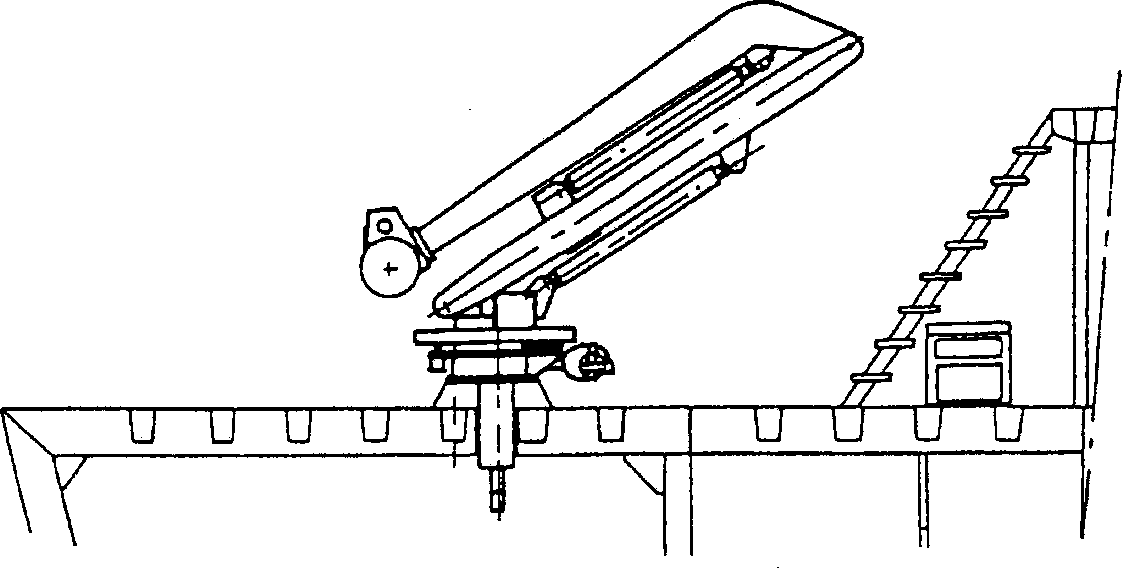
\includegraphics[width=.95\textwidth]{images/Grue}

\textit{Figure 1 : Implantation de la grue sur le pont d'un bateau}
\end{center}
\end{minipage} 

\vspace{.25cm}


\begin{minipage}[c]{.6\linewidth}
\begin{center}
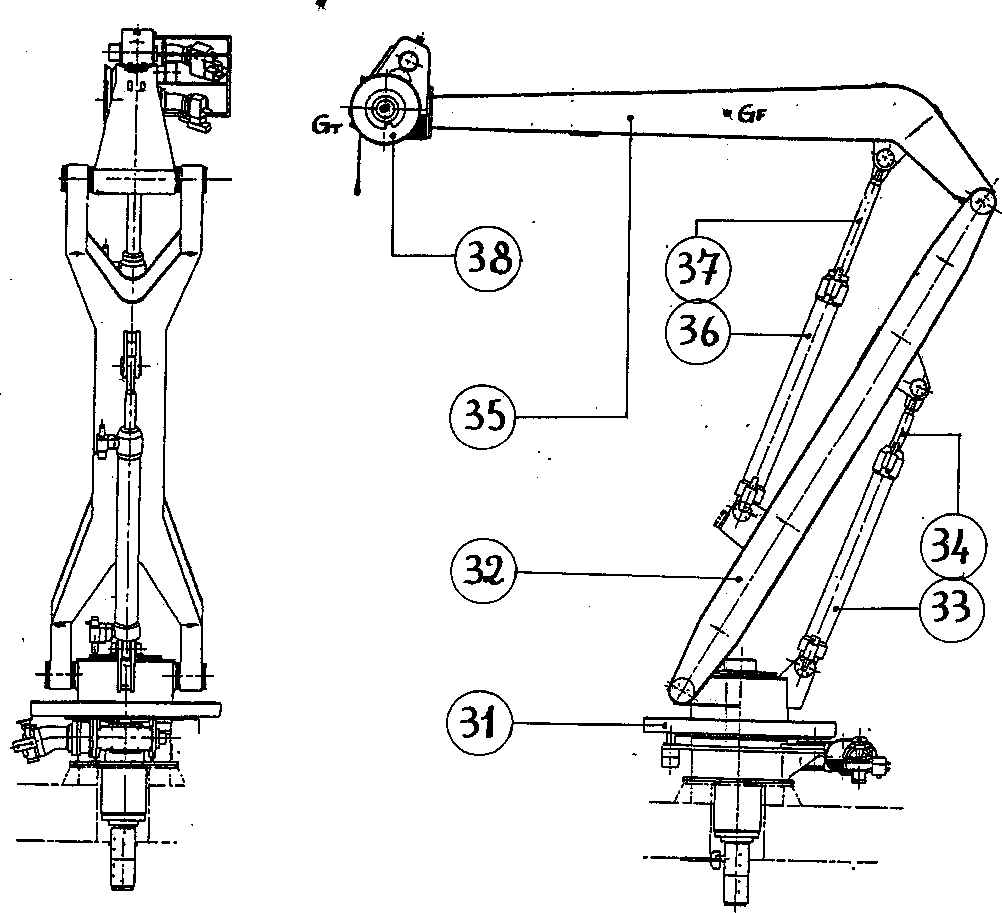
\includegraphics[width=.95\textwidth]{images/Grue_02}

\textit{Figure 2 : Vue générale -- échelle approximative 1:80}
\end{center}
\end{minipage} \hfill
\begin{minipage}[c]{.38\linewidth}

Le corps \textbf{31} pivote autour d'un axe vertical. Ce corps est solidaire d'une plateforme au dessous de laquelle un moto réducteur hydraulique et un couple pignon roue intérieure (ayant le diamètre approximatif de la plateforme) permettent d'actionner la rotation d'axe vertical.

Le portique \textbf{32}  est articulé sur \textbf{31}. Il est actionné par un vérin hydraulique. 

Une flèche \textbf{35} est articulée sur \textbf{32}. Elle est actionnée par un vérin hydraulique. 
\end{minipage}

\vspace{.25cm}

A l'extrémité de la flèche, un treuil \textbf{38} est équipé de deux moteurs hydrauliques réglables électroniquement afin d'assurer une tension constante du câble pour éviter les à-coups dus aux mouvements de la houle pendant l'ascension et la descente de la charge explosive. 


\begin{minipage}[c]{.49\linewidth}

L'ensemble est piloté à partir d'un pupitre portatif représenté sur la figure 3 :
\begin{itemize}
\item le levier à deux positions C2 commande la montée ou la descente de la flèche (vérin \textbf{36 -- 37});
\item le levier à deux positions C3 commande l'inclinaison du portique (vérin \textbf{33 --34});
\item les commandes de hissage et de rotation peuvent être combinés et sont regroupées sur le même levier;
\item le sélecteur C1 permet d'engager le système de suivi de houle ou de produire une descente à vide plus rapide.
\end{itemize}

\end{minipage} \hfill
\begin{minipage}[c]{.49\linewidth}
\begin{center}
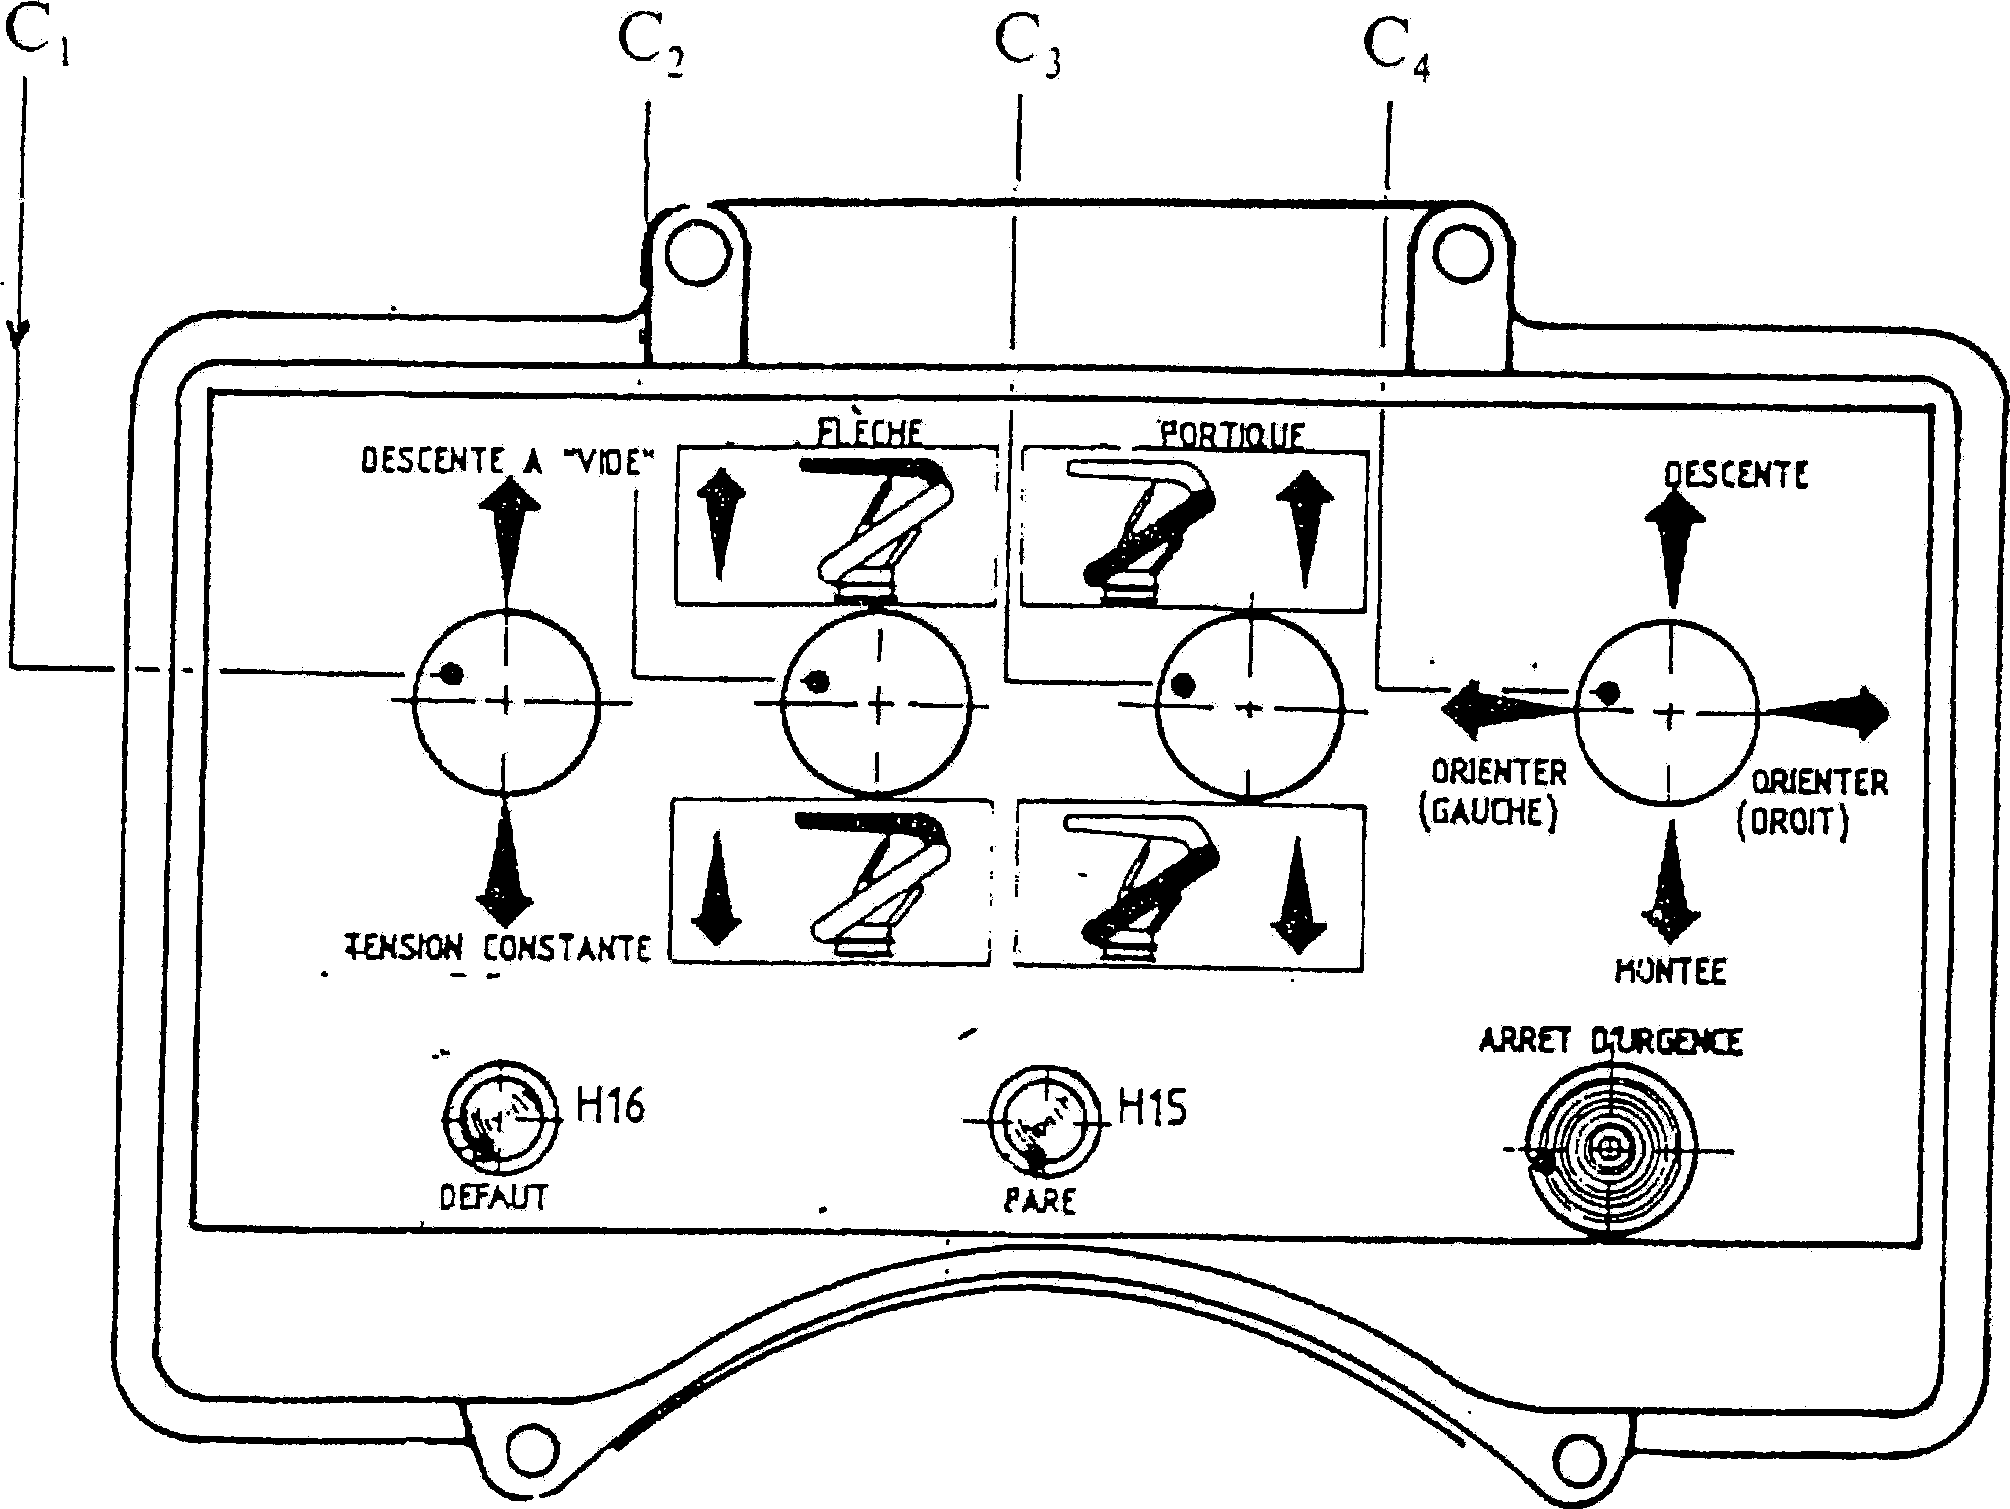
\includegraphics[width=.95\textwidth]{images/Pupitre}

\textit{Figure 3 : Pupitre de commande}
\end{center}
\end{minipage} 

\section{Fonctionnement du treuil}
La figure 4 présente les 3 vues extérieures du treuil. Celui-ci est boulonné à l'extrémité de la flèche. L'arbre de sortie supporte une bobine à enroulement spiral permettant des man\oe{}uvres rapides. Le treuil est muni de deux moteurs hydrauliques protégés des chocs par une structure tubulaire externe. 

\begin{center}
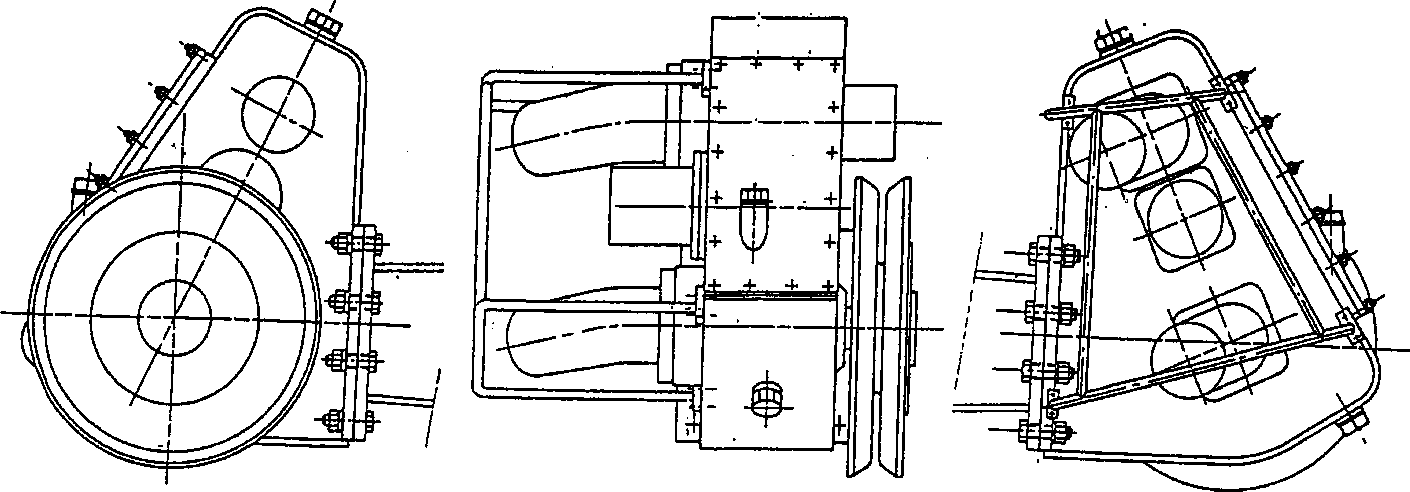
\includegraphics[width=.95\textwidth]{images/Treuil}

\textit{Figure 4 : Aspect extérieur du treuil -- Échelle approximative 1:14}
\end{center}

\begin{minipage}[c]{.49\linewidth}
Le treuil est schématisé sur la figure 5. Outre le dispositif réducteur de vitesse formé de deux trains d'engrenages cylindriques à denture droite, il est constitué des éléments suivants : 
\begin{itemize}
\item d'un moteur hydraulique principal [MP];
\item d'un moteur hydraulique de suivi de houle [MSH];
\item d'un système anti dévireur (roue libre);
\item d'un frein hydraulique à lamelles [FH];
\item d'un compte tours de fin de course [CT].
\end{itemize}

\end{minipage} \hfill
\begin{minipage}[c]{.49\linewidth}
\begin{center}
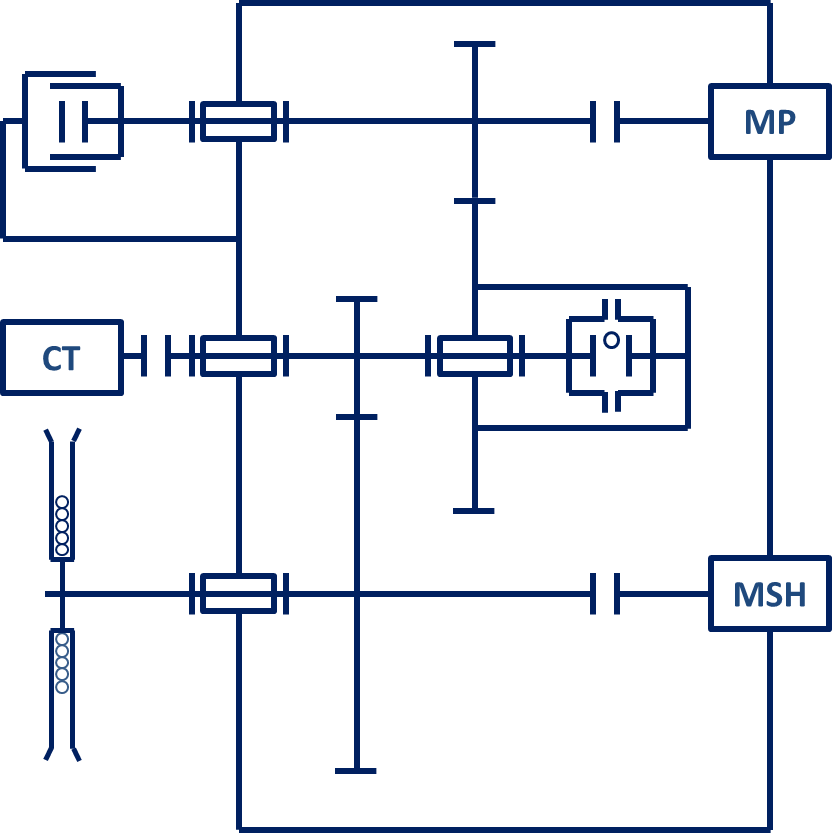
\includegraphics[width=.8\textwidth]{images/schema}

\textit{Figure 5 : Schéma du réducteur de treuil}
\end{center}
\end{minipage} 

\vspace{.25cm}


\begin{minipage}[c]{.49\linewidth}
Lors du fonctionnement en hissage (croquis 1 figure 6) ou en largage (croquis 2) sans houle, le [MSH] n'est pas mis en pression (sélecteur C1 au milieu). Il peut alors tourner dans les deux sens sans résistance notable. Il se comporte comme une pompe en circuit fermé. Seul le [MP] participe à la montée ou à la descente de la charge. 

Lors du largage avec mouvement de houle important (croquis 3), sélecteur C1 en bas, le [MP] est en mouvement de descente et le [MSH] est entraîné par la pression d'huile dans le sens de hissage pour maintenir une tension constante mais son couple est insuffisant pour soulever la charge. En revanche, sa position en prise directe sur l'arbre de la poulie d'enroulement permet d'enrouler rapidement le câble lorsque la charge est allégée par les efforts d'inertie dus au mouvement de la houle montante. 

En descendant, la houle augmente la tension du câble, le [MSH] est alors entraîné en sens contraire comme une pompe (croquis 4) et l'huile est alors renvoyée au réservoir basse pression.

Lors du largage du câble à vide (croquis 5), le [MSH] entraîne dans le sens de la descente. 

En cas de chute de pression hydraulique, le frein à lamelle bloque le réducteur. 

\end{minipage} \hfill
\begin{minipage}[c]{.49\linewidth}
\begin{center}
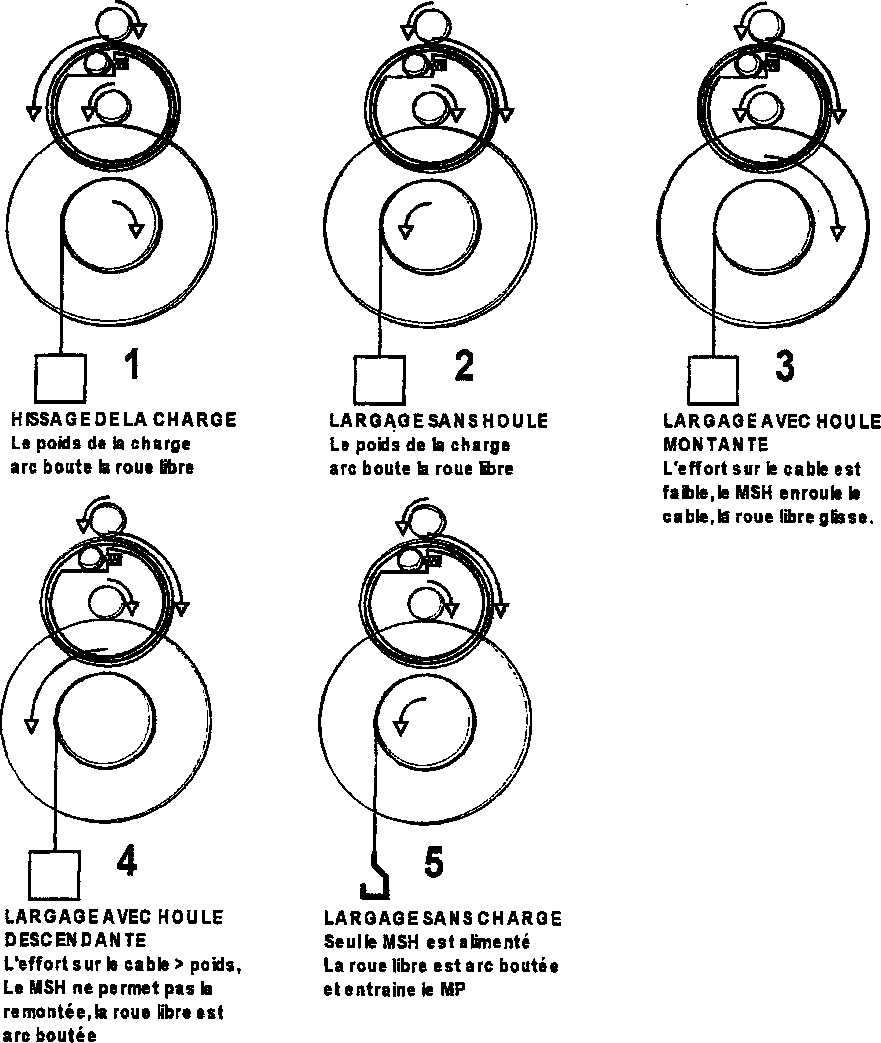
\includegraphics[width=\textwidth]{images/Treuil_02}

\textit{Figure 6 : Phases de fonctionnement}
\end{center}
\end{minipage} 


%\section{Étude de conception}

%On se propose dans un premier temps de concevoir le réducteur du treuil. %On donne pour cela sur le document annexe à l'échelle $1:2$, les dimensions exactes et les positions approximatives des éléments fondamentaux du réducteur. 

%\begin{itemize}
%\item Le moteur principal 2 est fixé au réducteur par 5 vis HM 12.
%\item Le moteur de suivi de houle 3 est de géométrie identique.
%\item Le compte tours 4 est fixé au réducteur par trois vis CHC M8.
%\item Le pignon arbré sur l'arbre d'entrée 5 a pour caractéristiques un module de 3 et 20 dents.
%\item Le pignon moulé 6 sur l'arbre intermédiaire a pour caractéristiques un module de 3 et 80 dents.
%\item Le pignon arbré 7 sur l'arbre intermédiaire a pour caractéristiques un module de 5 et 15 dents.
%\item La roue dentée 8 moulée présente sur l'arbre de sortie a pour caractéristiques un module de 5 et 70 dents.
%\item Une roue libre (à représenter en coupe médiane) est située entre 6 et 7.
%\item Le diamètre d'enroulement du câble sur la bobine est de 500\; mm.
%\item le diamètre minimum d'enroulement du câble est de 200 \; mm.
%\item L'enroulement est purement spiral.
%\item Le diamètre du câble en acier est de 10 mm.
%\item Le carter du réducteur(1a) est en fonte lamellaire moulée. 
%\item Il est constitué de deux parties dont un couvercle (1b) situé du côté des moteurs et du compte tour qui s'ouvre sur toute l'étendue de la face pour permettre le montage des constituants internes du réducteur.
%\item Le lubrification se fait par bain d'huile.
%\item Les formes externes ne doivent pas retenir l'eau des intempéries et doivent faciliter l'entretien périodique des installations de peinture. 
%\end{itemize}

\section{Conception de l'arbre primaire et du frein à lamelles}
Cette conception se fait à l'échelle 1 sur un format A3 horizontal. Les formes locales du carter et de son couvercle y seront définies. Les exigences à respecter sont listées dans le diagramme ci-dessous.
 
\begin{center}
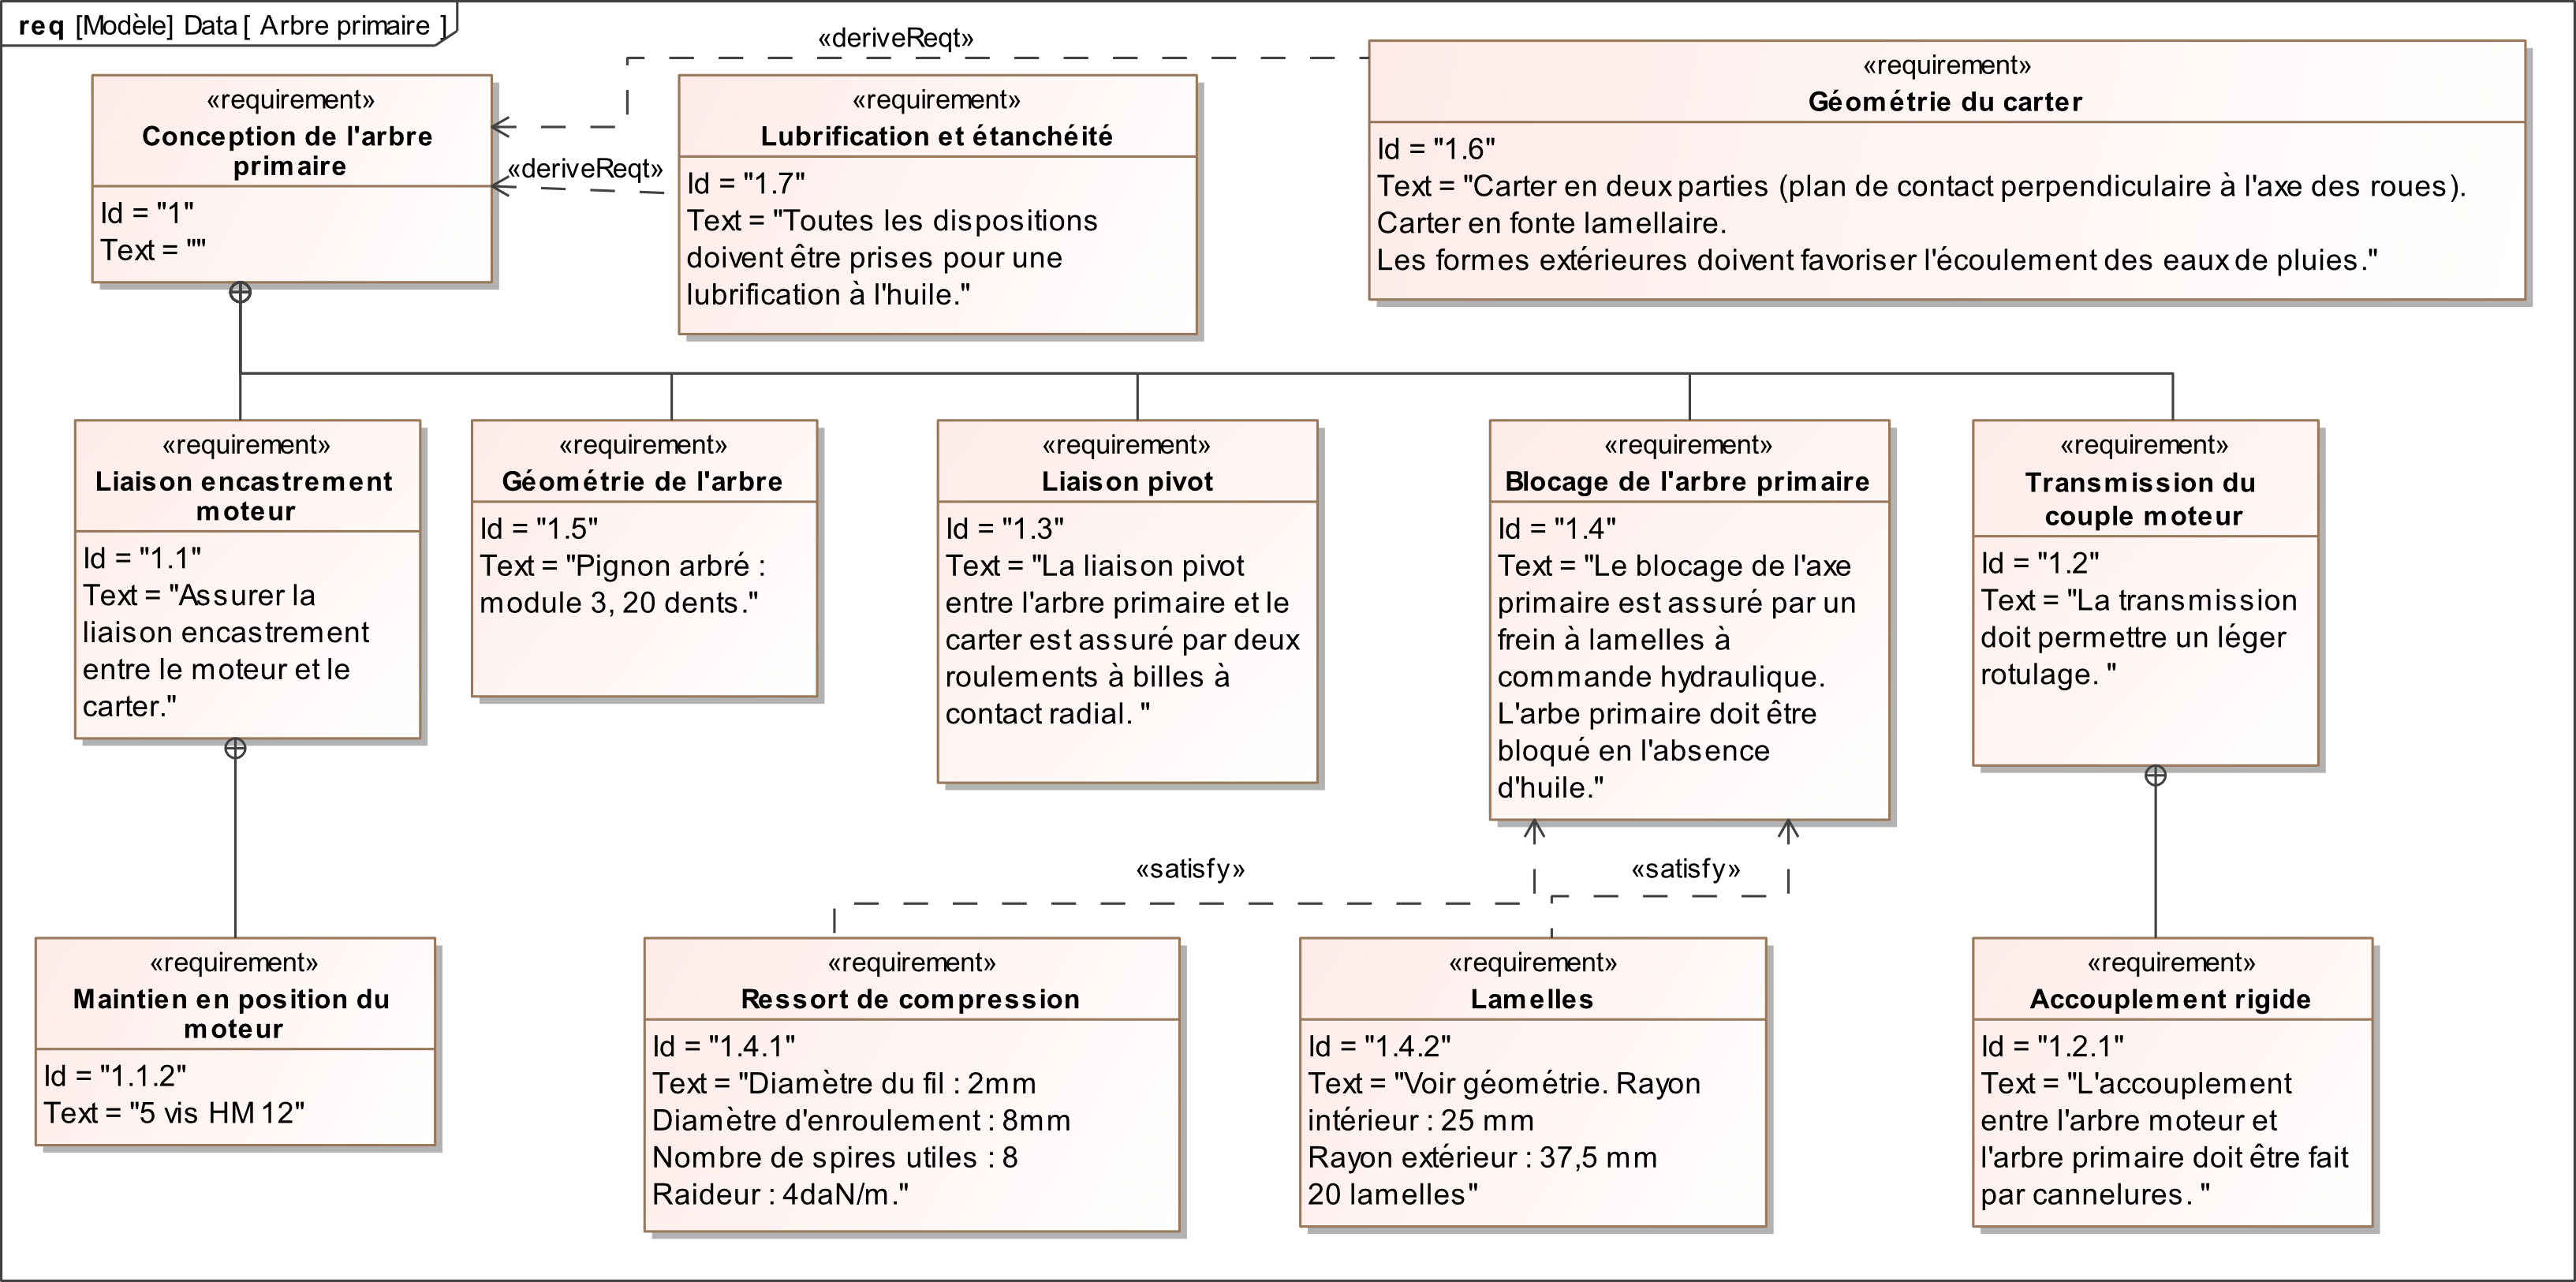
\includegraphics[width=\textwidth]{images/SysML/ArbrePrimaire.png}
\end{center}
%\begin{itemize}
%\item Liaison encastrement démontable du moteur principal 2 sur le couvercle du carter.
%\item Accouplement rigide avec léger rotulage autorisé entre l'arbre de sortie du moteur et l'arbre primaire 5. 
%\item Liaison pivot par roulements par rapport au carter et son couvercle.
%\item Le frein à lamelles à commande hydraulique. Il doit bloquer l'arbre primaire en l'absence de pression d'huile. On donne sur la figure 6 le schéma de principe de ce frein.
%\end{itemize}
%
%Les ressorts de compression sont constitués d'un fil d'acier au silicium de 2 mm de diamètre enroulé sur un diamètre moyen de 8 mm avec 8 spires utiles. Leur coefficient de raideur unitaire est de 4 daN/mm.

\subparagraph{}
\textit{Quel est le couple de freinage nécessaire pour bloquer la charge maximale avec une marge de sécurité de 30\%.}

\ifprof
\else
\fi


\subparagraph{}
\textit{Les représentations de face des lamelles étant fournies ci-dessous, rechercher un triplet optimal \{nombre de ressorts, nombre de lamelles, écrasement de précharge des ressorts\}. Le coefficient de frottement au niveau des lamelles sera minoré de 0,08.}

\subparagraph{}
\textit{Déterminer la section utile du piston pour désactiver le frein avec une pression de 20 bars.}

\subparagraph{}
\textit{Effectuer le dessin d'ensemble du montage de l'arbre primaire en coupe diamétrale.}


\begin{center}
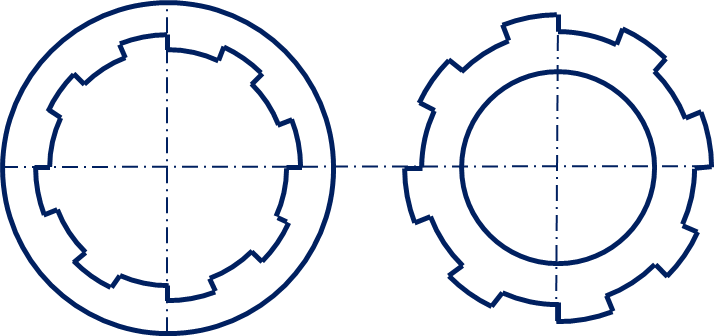
\includegraphics[width=.4\textwidth]{images/lamelles}\hfill
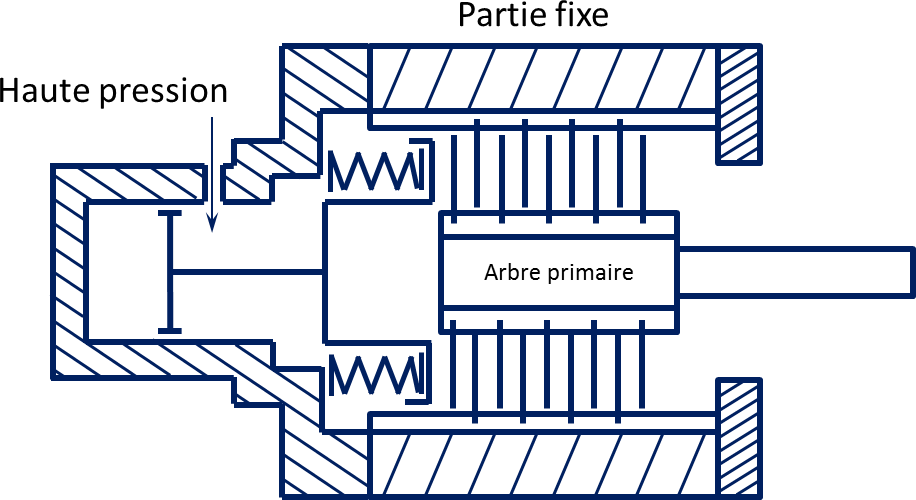
\includegraphics[width=.45\textwidth]{images/frein}

\textit{Figure 7 : Schémas des lamelles internes, externes et du frein à lamelles}
\end{center}

\section{Deuxième étape : Conception de l'arbre intermédiaire et de l'antidévireur}

Cette conception se fera sur un forma A3 tenu horizontalement à l'échelle 1. Les exigences à respecter sont données dans le diagramme ci-dessous.

\begin{center}
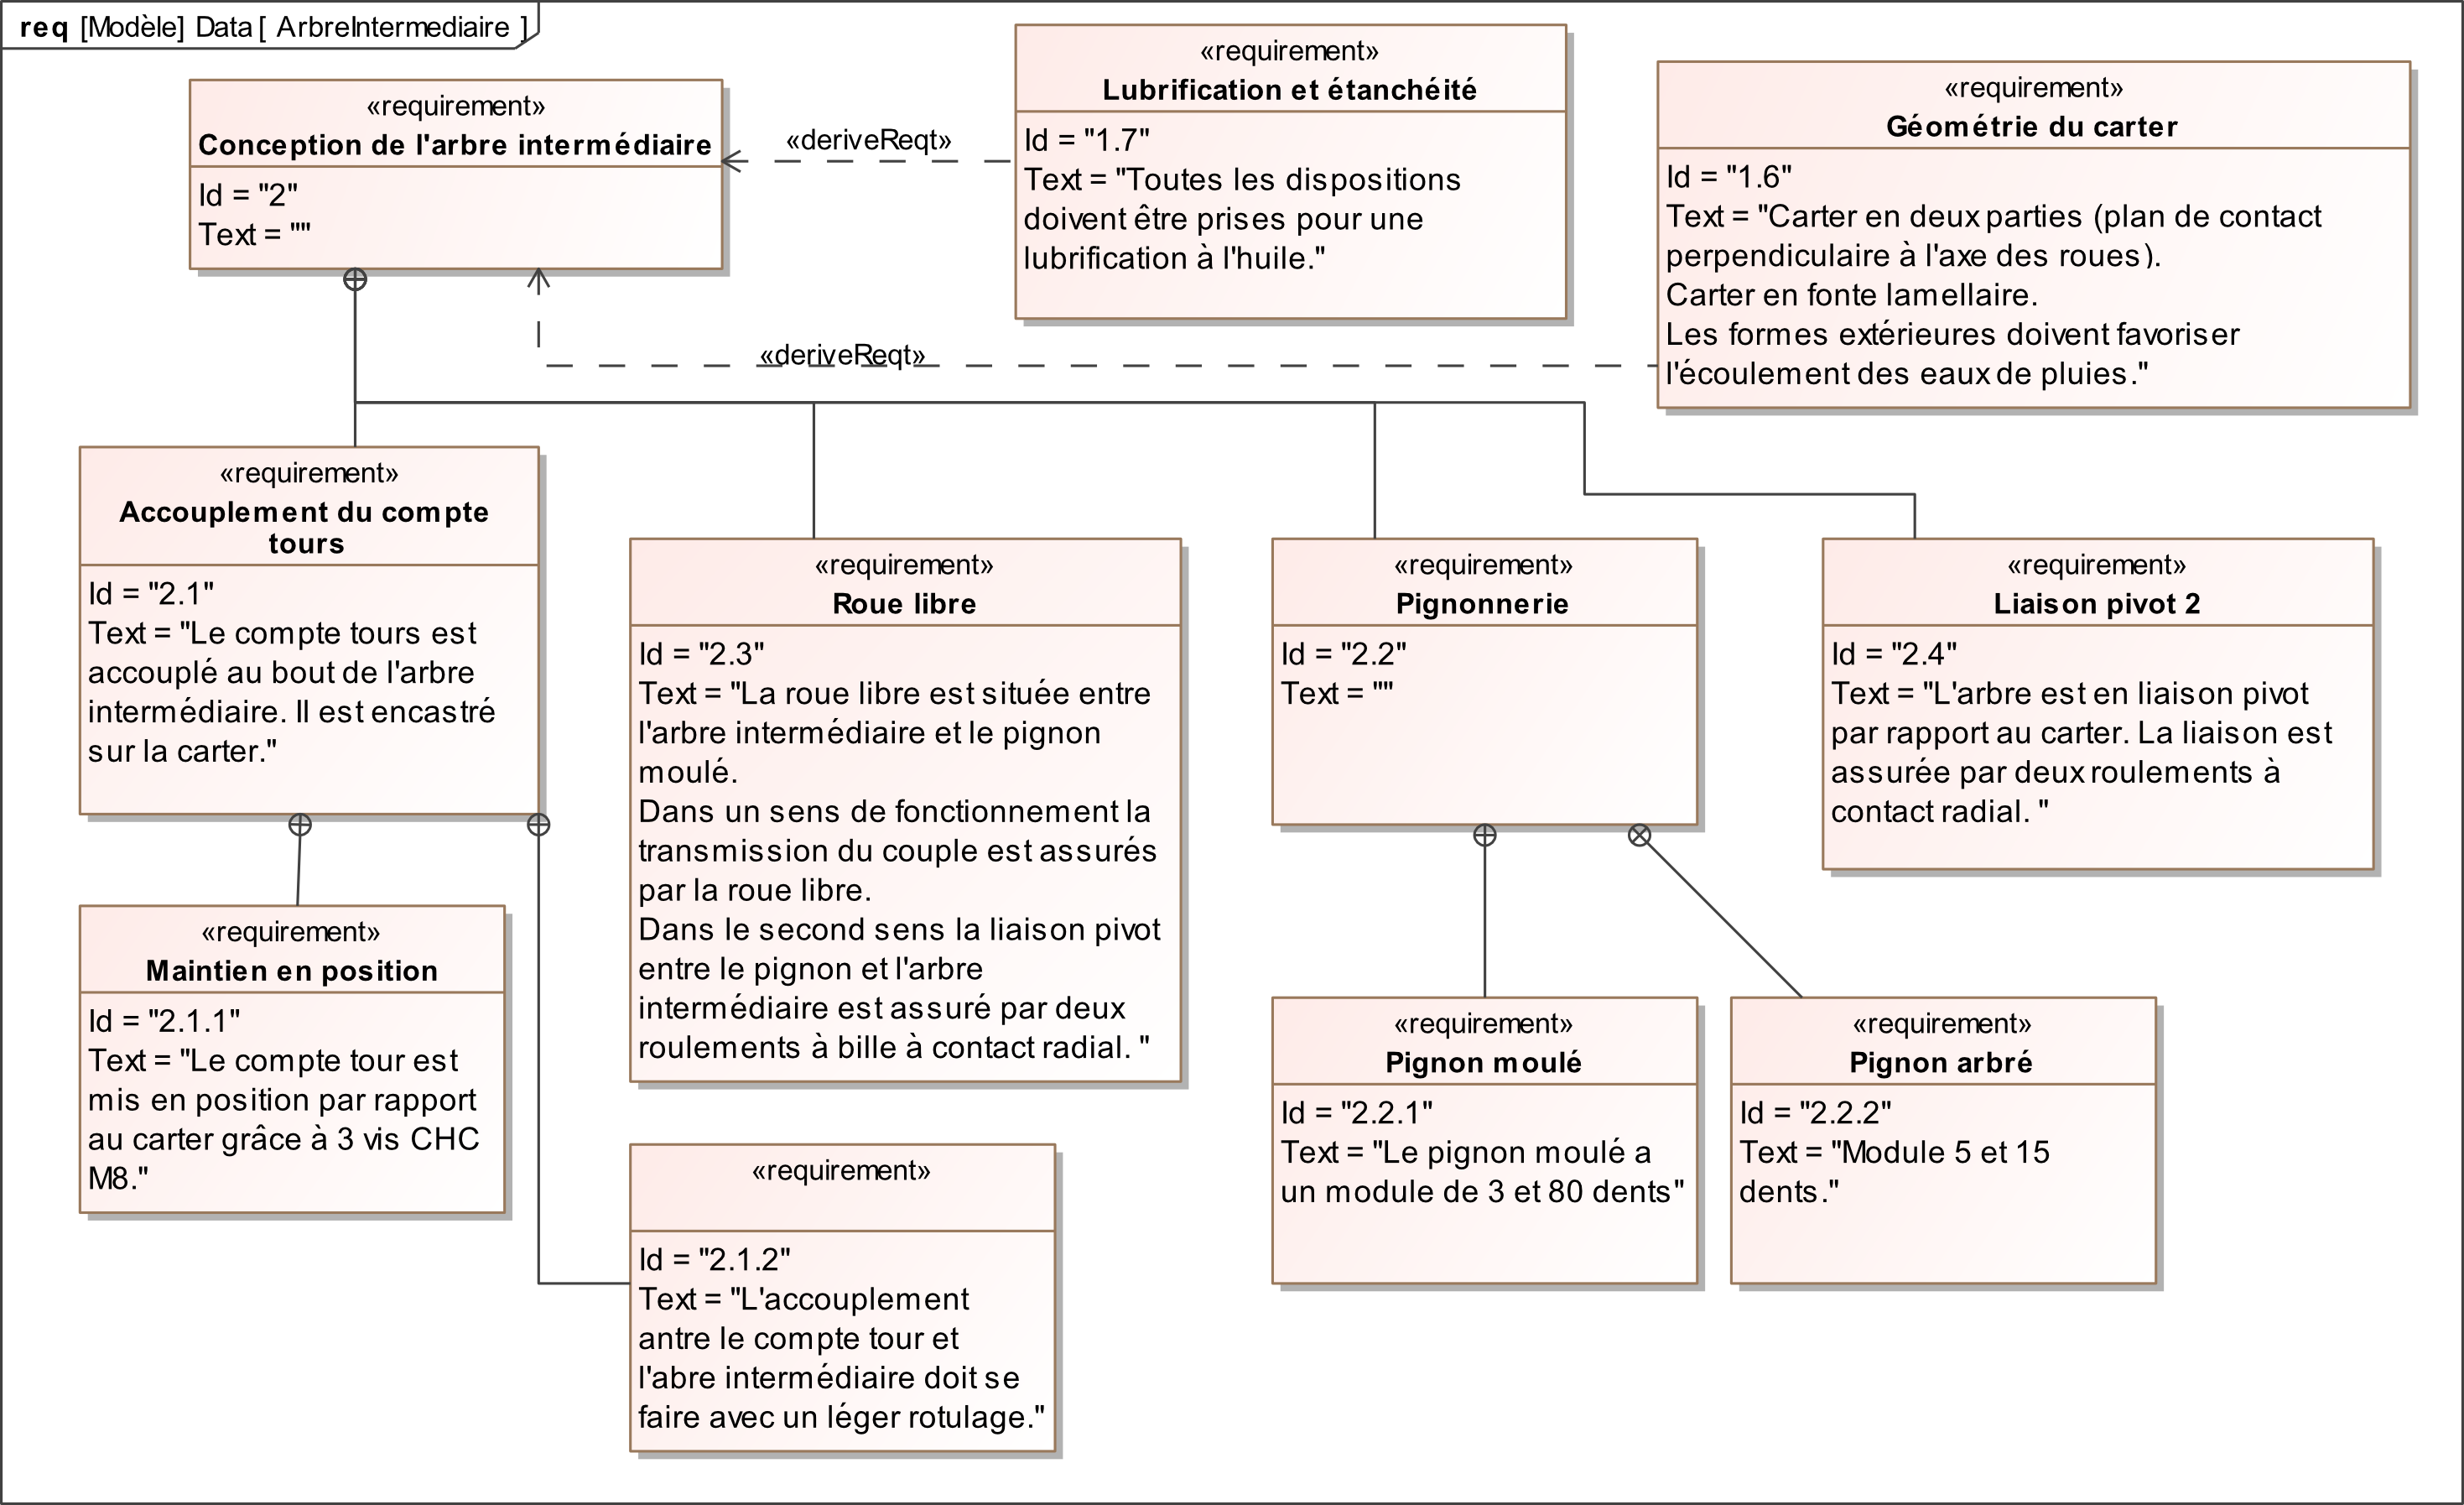
\includegraphics[width=\textwidth]{images/SysML/ArbreIntermediaire}
\end{center}

%La ligne d'arbre intermédiaire doit assurer plusieurs fonctions :
%\begin{itemize}
%\item liaison encastrement démontable du compte tours 4 sur le couvercle 1b du carter;
%\item accouplement rigide avec léger rotulage entre l'arbre du compte tours (4) et l'arbre intermédiaire (7) du réducteur de treuil;
%\item liaison pivot par deux roulements de l'arbre intermédiaire 7 par rapport au carter;
%\item guidage en rotation par deux roulements du pignon 6 par rapport à l'arbre 7
%\item dispositif antidévireur à rouleaux cylindriques entre 6 et 7. LA coupe BB du document annexe précise une architecture possible de ce dispositif. 
%\end{itemize}


\begin{minipage}[c]{.6\linewidth}
\subparagraph{}
\textit{Reproduire la figure ci-contre et représenter la condition d'équilibre limite du rouleau en phase d'arc boutement. Déduire l'expression de Hmini conditionnant le dégagement dans la bague interne en fonction de $R$ : rayon de la bague externe, $r$ rayon du rouleau et de $\varphi$ : angle de frottement.
Calculer la valeur de Hmin pour $R=47,5$, $r=5$ et $\tan\varphi = 0,07$.}

\end{minipage} \hfill
\begin{minipage}[c]{.38\linewidth}
\begin{center}
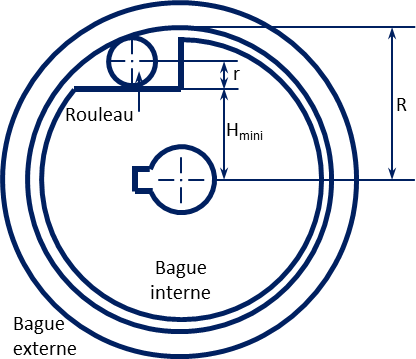
\includegraphics[width=.95\textwidth]{images/rouelibre}

\textit{Figure 8 : Étude de la roue libre}
\end{center}
\end{minipage} 


\subparagraph{}
\textit{Quel serait le couple transmis par la roue libre lors du soulèvement d'une charge de 7,5 kN avec une marge de 30\%.
La roue libre comporte 8 rouleaux de largeur $L=20\;mm$ et la hauteur du dégagement est $H=37,2\; mm$. Déterminer la valeur de la densité linéique d'effort de contact entre un rouleau et la bague externe dans les conditions ci-dessus.
Proposer des matériaux cohérents pour les rouleaux et les bagues de l'antidévireur.}


\subparagraph{}
\textit{Effectuer le dessin d'ensemble du montage de l'arbre intermédiaire de la roue libre en coupe diamétrale.}


\section{Troisième étape : conception de l'arbre de sortie du réducteur}

Cette conception se fera sur format A3 en tenant compte des éléments précédents. Les exigences à respecter sont listées dans le diagramme des exigences suivant. 

\begin{center}
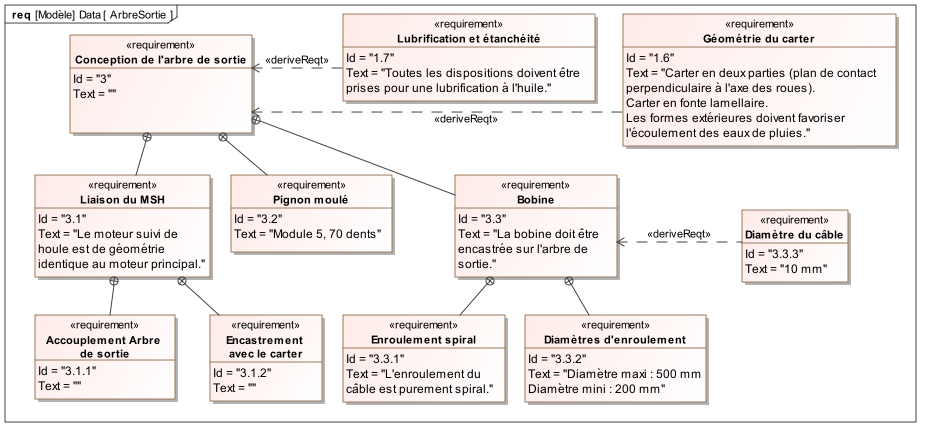
\includegraphics[width=\textwidth]{images/SysML/ArbreSortie}
\end{center}




\subparagraph{}
\textit{Déterminer le nombre de tours $N$ que le câble peut effectuer autour de la poulie. 
Déterminer la longueur d'enroulement du câble au ième tour à partir du début de l'enroulement de la bobine vide.
Déduire la longueur totale $L$ du câble qui peut être enroulé sur la bobine pleine.}

\subparagraph{}
\textit{Effectuer le graphe de la vitesse d'enroulement du câble en fonction du temps pour une vitesse de moteur principal de 1000 tours/min.
L'accélération qui en découle a-t-elle une influence importante sur la tension du câble ?}

\subparagraph{}
\textit{Effectuer le dessin d'ensemble du montage de l'arbre de sortie et de la bobine en coupe diamétrale.}


\section{Quatrième étape :  conception de l'articulation du portique par rapport à la flèche}

Cette conception se fera sur deux formats A3. Une première vue à l'échelle 1/4 donnera l'allure de l'ensemble de la liaison articulation, mais cette représentation s'avère insuffisante pour fournir les détails structurels et dimensionnels de l'étude. Ces détails seront donc dessinés à l'échelle 1 sur une seconde feuille, pour une partie seulement de la liaison. 

La masse de la flèche est évaluée à 260 kg, celle du treuil à 100 kg. Les centres de gravité sont représentés sur la figure 1. 

\subparagraph{}
\textit{Déterminer par une méthode graphique l'effort appliqué sur cette articulation lorsque la grue est en surcharge de 30\%.}

\subparagraph{}
\textit{Évaluer alors la pression de contact dans les paliers. }

\subparagraph{}
\textit{Effectuer la cotation fonctionnelle complète de l'ensemble des pièces constituants cette articulation (dimensions linéaires, défauts de forme et de position, états de surface).}


\section*{Annexes}

\subsection*{Couple transmissible par adhérence dans un embrayage à disque ou dans un frein}


\begin{minipage}[c]{.3\linewidth}
\begin{center}
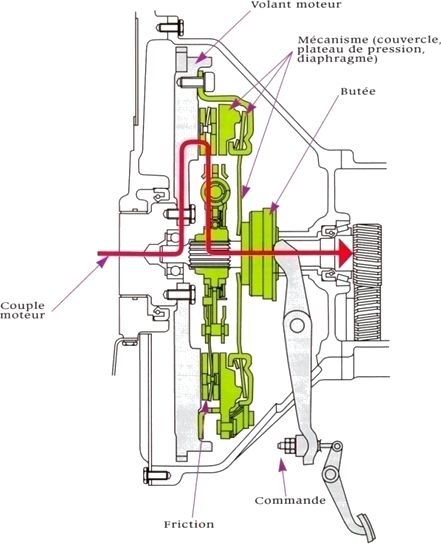
\includegraphics[width=.95\textwidth]{images/embrayage}
\end{center}
\end{minipage}\hfill
\begin{minipage}[c]{.65\linewidth}
\begin{center}
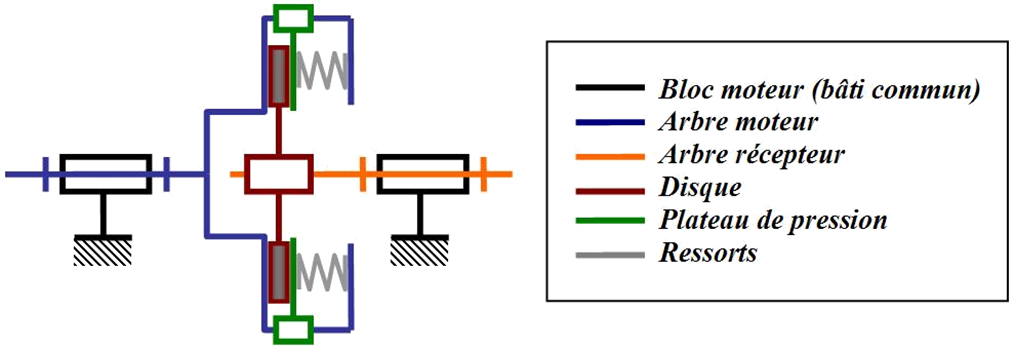
\includegraphics[width=.95\textwidth]{images/embrayage2}
\end{center}
\end{minipage}


On donne $k$ la raideur des ressorts, $f$ le facteur de frottement entre les le disque et l'arbre moteur, $r$ le petit rayon de la couronne et $R$ le grand rayon de la couronne. Calculer le couple transmissible par adhérence entre l'arbre moteur et le disque. On fera l'hypothèse que l'action créée par les ressorts sur le plateau de compression est uniforme. 

\textbf{Expression du couple infinitésimal : }$
d\vectm{\text{Plateau}}{\text{Disque}}{O} =
d\vectm{P}{D}{O} =  \vect{OM}\wedge d\vectf{P}{D}
$

\textbf{Expression de la résultante infinitésimale : } 
$d\vectf{P}{D} = d\vect{N(P\rightarrow D)}+d\vect{T(P\rightarrow D)}$

\textbf{Expression de l'effort normal : }
$ d\vect{N(P\rightarrow D)} = p \vect{n} d\mathcal{S} = -p \vect{z} d\mathcal{S} $

\textbf{Expression de l'unité de surface : }
$ d\mathcal{S} = \rho d\theta d\rho $

\textbf{Expression de l'effort tangentiel : } d'après le modèle de Coulomb, on commence par identifier le vecteur $\vectv{M}{D}{P}$.
Le vecteur tangentiel est donc opposé à ce dernier. A la limite du glissement on a alors : 
$$
d\vect{T(P\rightarrow D)} = -f ||d\vect{N(P\rightarrow D)}|| \vect{v}    = fp d\mathcal{S}\vect{v}
$$

\textbf{Calcul final :} on note $\vect{OM}=\rho\vect{u}$ :

\begin{eqnarray*}
\vectm{O}{P}{D}  
&=& d\vectm{O}{P}{D}  =  \int \vect{OM}\wedge d\vectf{P}{D} = \int \rho\vect{u} \wedge \left( d\vect{N(P\rightarrow D)}+d\vect{T(P\rightarrow D)} \right)\\
&=& \int \rho\vect{u} \wedge \left( -p \vect{z} d\mathcal{S} +fp d\mathcal{S}\vect{v} \right) =  \iint p\rho\vect{v} d\mathcal{S} +\iint pf\rho  \vect{z}d\mathcal{S} \\
& =& \iint p\rho\vect{v} \rho d\theta d\rho +\iint pf\rho  \vect{z}\rho d\theta d\rho \\
\end{eqnarray*}

\begin{eqnarray*}
\iint p\rho\vect{v} \rho d\theta d\rho &=& \iint p\rho\left(\cos\theta\vect{y}-\sin\theta\vect{x} \right) \rho d\theta d\rho =\iint p\rho\cos\theta\vect{y}  \rho d\theta d\rho-\iint p\rho \sin\theta\vect{x}  \rho d\theta d\rho \\
&= &p \vect{y}  \int\limits_{r}^{R} \int\limits_{0}^{2\pi}\cos\theta d\theta \rho^2 d\rho- p\vect{x}\int\limits_{r}^{R} \int\limits_{0}^{2\pi} \sin\theta  \rho^2 d\theta d\rho = p \left[ \sin\theta\right]_{0}^{2\pi}\left[ \dfrac{1}{3}\rho^3\right]_{r}^{R}\vect{y}
 -p \left[ -\cos\theta\right]_{0}^{2\pi}\left[ \dfrac{1}{3}\rho^3\right]_{r}^{R}\vect{x} = \vect{0}
\end{eqnarray*}

\begin{eqnarray*}
\iint pf\rho^2 \vect{z} d\theta d\rho =
pf \left[ \theta\right]_{0}^{2\pi}\left[ \dfrac{1}{3}\rho^3\right]_{r}^{R} \vect{z}
= pf2\pi \dfrac{R^3-r^3}{3} 
\end{eqnarray*} 

Enfin, en notant $F_r$ l'effort (uniformément réparti) exercé par le ressort sur toute la couronne, on a donc :
$$
p=\dfrac{F_r}{\pi \left(R^2-r^2 \right)}
$$

Au final : 

$$ \vectm{O}{P}{D}  
= f\dfrac{2}{3} \dfrac{R^3-r^3}{R^2-r^2} F_r
$$


Le facteur de frottement ne dépend pas de la pression de contact entre deux solides.

\begin{center}
\begin{tabular}{|c||c|c||c|c|}
\hline
\multirow{2}{*}{Matériaux} 
& \multicolumn{2}{c||}{Facteur d'adhérence} & \multicolumn{2}{c|}{Facteur de glissement} \\
\cline{2-5}
& Sec & Lubrifié & Sec & Lubrifié \\
\hline
\hline
Acier / Acier & 0,2 à 0,3 & 0,15 à 0,2 & 0,2 & 0,12 \\ \hline
Acier / Fonte & 0,2 & 0,12 à 0,2 & 0,15 & 0,08 \\ \hline
Acier / Bronze & 0,2 & 0,15 à 0,2 & 0,2 & 0,12 \\ \hline
Acier / Métal fritté &  & 0,1 à 0,18 & 0,1 à 0,12 & 0,03 à 0,06 \\ \hline
Acier / Garniture de friction & 0,3 à 0,4 &  & 0,25 à 0,35 &  \\ \hline
Acier / Graphite &  & 0,1 &  & 0,09 \\ \hline
Acier / Palier PTFE & 0,08 à 0,4 &  & 0,02 à 0,08 & 0,003 à 0,05 \\ \hline
Pneu neuf / Route & 1 & 0,6  & 0,5 à 0,6  & 0,2 à 0,5\\ \hline
\end{tabular}
\end{center}



\subsection*{Esquisse du moteur hydraulique et du compte tours}

\begin{center}
\rotatebox{270}{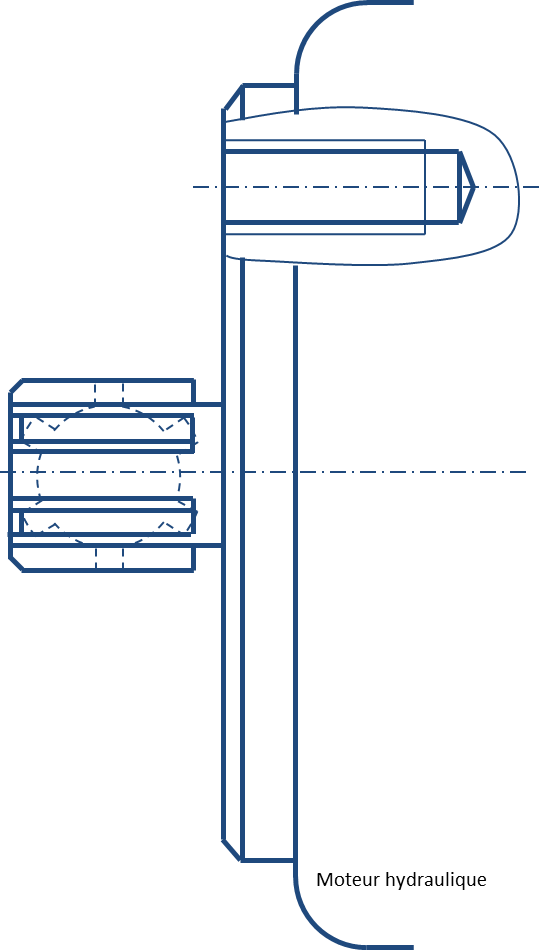
\includegraphics[height=.95\textwidth]{images/MoteurHydraulique}}

\rotatebox{270}{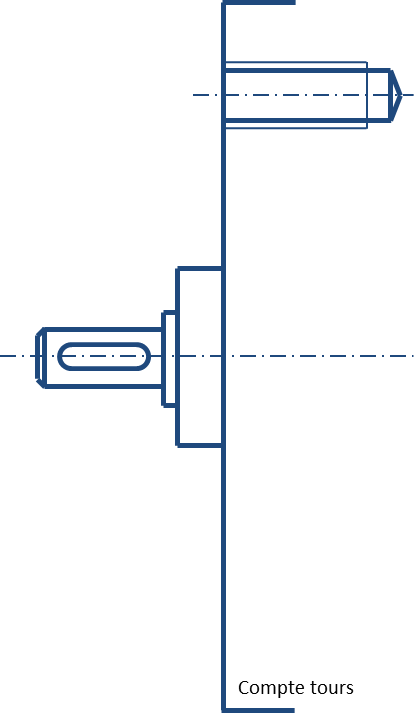
\includegraphics[height=.8\textwidth]{images/CompteTours}}
\end{center}

\end{document}


